\documentclass[11pt]{article}
\usepackage[margin=1in]{geometry}
\usepackage{graphicx}
\usepackage{amsmath,amssymb}
\usepackage{booktabs}
\usepackage[numbers,sort&compress]{natbib}  % MRM: numbered (Vancouver) references
\usepackage{xcolor}
\usepackage[colorlinks=true,linkcolor=blue,citecolor=blue,urlcolor=blue]{hyperref}
\usepackage{microtype}
\usepackage{caption}
\emergencystretch=2em

\newcommand{\Dstar}{D^{*}}
\newcommand{\unit}[1]{\,\mathrm{#1}}
% Multi-seed empirical [5,95] confidence band (16 seeds; see Sec.~\ref{sec:consistency}).
\newcommand{\band}[2]{{\scriptsize\,$[#1,\,#2]$}}

\title{\textbf{Distribution-Free Conformal Coverage for IVIM Parameter
Maps, and the Identifiability Wall in the Pseudo-Diffusion Compartment}}
\author{Avery Karlin\\[3pt]
\small Department of Applied Physics and Applied Mathematics, Columbia University, New York, NY, USA\\[1pt]
\small Department of Computer Science, University of Colorado Boulder, Boulder, CO, USA\\[1pt]
\small The Annealing Signet Institute\\[3pt]
\small ORCID: \href{https://orcid.org/0000-0003-3848-6782}{0000-0003-3848-6782}}
\date{}

\begin{document}
\maketitle

\begin{abstract}
\noindent
\textbf{Purpose:} To characterize the identifiability limit governing per-voxel
uncertainty in the ill-posed pseudo-diffusion compartment ($\Dstar$) of intravoxel
incoherent motion (IVIM) imaging, using distribution-free conformal prediction both
as the finite-sample coverage tool model-based uncertainty quantification (UQ) lacks
and a lens on where label-free conditioning fails.

\noindent
\textbf{Methods:} On a controlled, seeded synthetic cohort, we compare
split-conformal and conformalized quantile regression (CQR) against four model-based
baselines (probabilistic network, mixture-density ensemble, deep ensemble, Bayesian
MCMC), measuring marginal and (SNR $\times$ true-$\Dstar$-tercile) conditional
coverage with 16-seed confidence bands; a Cram\'er--Rao (CRLB) analysis
diagnoses the residual gap.

\noindent
\textbf{Results:} The failure is conditional: the high-$\Dstar$ regime
under-covers for every label-free method tested -- the IVIM instance of the
impossibility of distribution-free conditional coverage~\citep{barber2021limits};
the Cram\'er--Rao bound reaches the regime-bin width here, a concomitant diagnostic,
not the cause. Conformal methods restore near-nominal marginal coverage
($|\text{gap}|\le 0.024$), and conformalizing the MDN is the sharpest valid recipe
($0.65$--$0.77\times$ pure-CQR width). The wall replicates on OSIPI ground truth,
under a non-bi-exponential generator, and a clinically realistic prior.

\noindent
\textbf{Conclusion:} High-$\Dstar$ conditional coverage is unrecoverable by the
label-free methods tested; we characterize this limit, not solve it, and make no
in-vivo coverage claim. In practice this is a triage rule: trust the well-identified
diffusion map $D$, read high-$\Dstar$ as unresolved, and rely on the label-free
deployment monitor as a safeguard.
\end{abstract}

\vspace{0.5em}
\noindent\textbf{Keywords:} intravoxel incoherent motion (IVIM); uncertainty
quantification; conformal prediction; identifiability; pseudo-diffusion;
quantitative MRI.

\vspace{0.5em}
\noindent\textbf{Word count (Introduction--Conclusions):} 4,933
(\texttt{texcount} ``Words in text''; excludes title page, abstract, section
headings, float captions, tables, and references). Confirmed $\le 5000$.

\section{Introduction}
IVIM imaging~\citep{lebihan1988} separates microcirculatory perfusion from tissue
diffusion by fitting the bi-exponential signal
\begin{equation}
\frac{S(b)}{S_0} = f\,e^{-b\Dstar} + (1-f)\,e^{-bD},
\label{eq:ivim}
\end{equation}
where $b$ is the diffusion weighting (s/mm$^2$), $D$ the tissue diffusion
coefficient, $\Dstar \gg D$ the pseudo-diffusion coefficient, and $f$ the
perfusion fraction. Equation~\eqref{eq:ivim} is notoriously ill-posed: $\Dstar$ is
poorly constrained because the fast-decaying perfusion term contributes only at
low $b$, and small perfusion fractions make it nearly unidentifiable. Clinical use
of IVIM parameter maps therefore demands trustworthy \emph{per-voxel uncertainty},
not just point estimates.

\subsection{Related work}\label{sec:related}
\textbf{IVIM estimation and its model-based uncertainty.} The bi-exponential fit is
long known to be ill-posed in the perfusion compartment; a substantial literature
addresses the resulting $\Dstar$ instability through segmented and constrained
non-linear least squares, multi-algorithm comparisons documenting wide
between-method disagreement~\citep{gurneychampion2018}, Cram\'er--Rao-guided
acquisition design~\citep{lemke2011}, and supervised or physics-informed deep
networks~\citep{barbieri2020,kaandorp2021,mastropietro2022} that sharpen point
estimates without certifying their own reliability. Uncertainty quantification for
IVIM is accordingly \emph{model-based}: Bayesian fitting with informative or spatial
priors~\citep{gustafsson2018,spinner2021}, posterior estimation with explicit
uncertainty~\citep{zhang2019}, and, most comprehensively, deep ensembles of
mixture-density networks that split aleatoric and epistemic
uncertainty~\citep{casali2026}. Every such method places a distribution over
parameters and reads intervals from it; none carries a finite-sample,
distribution-free coverage guarantee, and the most thorough documents residual
overconfidence in $\Dstar$~\citep{casali2026}.

\textbf{Conformal prediction and imaging.} Conformal
prediction~\citep{vovk2005,lei2018,angelopoulos2023} yields finite-sample,
distribution-free \emph{marginal} coverage for \emph{any} base predictor under
exchangeability -- a biased base only widens the interval, it does not break
coverage -- and conformalized quantile regression (CQR)~\citep{romano2019} makes the
intervals input-adaptive; the framework extends to covariate
shift~\citep{tibshirani2019,barber2023} and localized/conditional
guarantees~\citep{guan2023,gibbs2023}. Distribution-free \emph{conditional} coverage
is, however, known to be unattainable in general without distributional
assumptions~\citep{barber2021limits} -- exactly the boundary that surfaces, in
IVIM-specific form, when the conditioning axis is the unidentifiable $\Dstar$
regime. Conformal UQ has been applied to distribution-free image-to-image
regression~\citep{angelopoulos2022}, fairness in medical-imaging
predictors~\citep{lu2022}, and -- closest to this work -- quantitative-MRI
relaxometry and field mapping via CQR~\citep{birk2024}, but never to the ill-posed
IVIM inverse problem and never benchmarked head-to-head against model-based IVIM UQ.

This paper closes that gap and, in doing so, \emph{reframes} the question. We began
with the hypothesis that conformal prediction's advantage would concentrate in the
unstable $\Dstar$ (and secondarily $f$) compartment, exactly where model-based UQ
is documented weak. The data reject the \emph{marginal} form of that hypothesis and
replace it with a sharper, IVIM-specific finding. Our contributions are:
\begin{enumerate}
\item \textbf{An identifiability limit, characterized in IVIM.} The genuine
IVIM-specific phenomenon is conditional: the high-$\Dstar$ regime under-covers
across eleven label-free conditioning methods
(Secs.~\ref{sec:conditional}--\ref{sec:identifiability}). We separate two facts the
regime ties together: (i) coverage conditional on the true $\Dstar$ regime is not
label-free-attainable because that regime is a latent axis the data do not reveal --
the IVIM instance of the known impossibility of distribution-free conditional
coverage~\citep{barber2021limits}; and (ii) independently, a Cram\'er--Rao (CRLB)
analysis shows $\Dstar$ is poorly point-identified in the same regime (the CRLB
reaches the regime-bin width). The conformal layer renders the conditional limit
measurable, and our evidence is that it is a property of the perfusion-estimation
problem, not our estimator: it persists for a deliberately biased shrinkage
estimator and replicates under a non-bi-exponential (velocity-dispersion) generator
(Secs.~\ref{sec:dissociation-shrinkage},~\ref{sec:altmodel}), with the off-model
validity envelope charted in Sec.~\ref{sec:envelope}.
\item \textbf{The first conformal/CQR coverage for IVIM, benchmarked.} We bring
distribution-free conformal prediction to the ill-posed IVIM inverse problem with
validated finite-sample marginal coverage for $(D,\Dstar,f)$, and the first
head-to-head benchmark against four model-based UQ baselines -- showing model-based
IVIM UQ is overconfident \emph{broadly} (not $\Dstar$-specifically) and that
conformalizing a strong model-based base is the sharpest valid recipe
(Secs.~\ref{sec:methods},~\ref{sec:marginal}).
\item \textbf{Robustness, acquisition-sensitivity, and an honest in-vivo
demonstration}: weighted conformal recovers covariate shift but not
forward-model misspecification, an observable monitor flags deployment-validity
breaks before coverage fails, the wall is robust to the b-value scheme, and the
in-vivo component is explicitly qualitative with no coverage claim
(Secs.~\ref{sec:robustness}--\ref{sec:invivo}).
\end{enumerate}
Every number in this paper traces to a gated, seeded checkpoint output, verified by a
machine-checked consistency report (Sec.~\ref{sec:consistency}).

\section{Methods}
\label{sec:methods}

\paragraph{Forward model and synthetic cohort.}
Conformal calibration requires \emph{labeled} data, which in-vivo IVIM cannot
provide, so the cohort is synthetic and built from our own implementation of
Eq.~\eqref{eq:ivim} with Rician noise ($\sigma = S_0/\mathrm{SNR}$). Parameters are
drawn uniformly from published abdominal ranges: $D\in[0.5,3.0]\times10^{-3}$,
$\Dstar\in[10,100]\times10^{-3}\unit{mm^2/s}$, $f\in[0.05,0.40]$; SNR is drawn from
$\{10,20,30,50,100\}$; the b-value scheme has 22 values
($0,10,\dots,100,120,\dots,200,300,\dots,800\unit{s/mm^2}$), dense at low $b$ to
separate $\Dstar$. The three splits (train/calibration/test $=4000/2000/3000$) are
i.i.d.\ draws from one seed (\texttt{20260613}), making calibration and test
exchangeable. On clean (noise-free) signals the generator and the non-linear
least-squares (NLLS) estimator recover the truth to a maximum relative error of
$2.07\times10^{-7}$, confirming label self-consistency.

\paragraph{Conformal intervals.}
For a base point predictor $\hat\theta$, \emph{split conformal} uses calibration
nonconformity scores $s_i = |\theta_i - \hat\theta_i|$ and the radius
$q=\lceil(n{+}1)(1-\alpha)\rceil$-th smallest score, giving
$[\hat\theta - q,\ \hat\theta + q]$ with marginal coverage in
$[1-\alpha,\,1-\alpha+1/(n{+}1)]$. \emph{CQR}~\citep{romano2019} conformalizes a
gradient-boosted quantile-regression base. We also \emph{conformalize model-based}
bases by treating their predictive quantiles as the CQR band, which restores the
guarantee while keeping the model's sharpness.

\paragraph{Model-based baselines.}
Four standard, independent model-based UQ baselines emit per-parameter intervals on
the matched cohort: a single probabilistic NN (Gaussian NLL head); a deep ensemble
of mixture-density networks~\citep{bishop1994,lakshminarayanan2017} following the
Casali approach~\citep{casali2026} with an aleatoric/epistemic split; a plain deep
ensemble of point regressors (epistemic-only; deliberately weak, retained as a
worst-case base for the conformal layer rather than as a representative model-based
method); and a per-voxel
Bayesian fit by component-wise adaptive Metropolis (fed the true noise level, so it
is evaluated at its best). This work is deliberately independent of normalizing-flow /
simulation-based posterior estimation and does not use it as a baseline.

\paragraph{Conditional coverage and the identifiability diagnostic.}
We measure coverage on a (true-$\Dstar$ tercile $\times$ SNR) grid -- the terciles
are a diagnostic only; the true $\Dstar$ is unknown at test time. To ask whether a
residual gap is a method failure or an information limit, we compute the Fisher
information for $\theta=(D,\Dstar,f,S_0)$ under the high-SNR Gaussian approximation,
$\mathcal{I}=J^\top J/\sigma^2$ with $J$ the signal Jacobian, and the
Cram\'er--Rao lower bound (CRLB)~\citep{cramer1946}
$\mathrm{CRLB}(\theta_k)=\sqrt{[\mathcal{I}^{-1}]_{kk}}$.

\paragraph{Robustness tooling.}
To stress exchangeability we use \emph{weighted / nonexchangeable
conformal}~\citep{tibshirani2019,barber2023} (importance weights
$w(x)=\mathrm{d}P_{\text{test}}/\mathrm{d}P_{\text{cal}}$ from a domain classifier on
observable features) and \emph{localized}~\citep{guan2023} /
\emph{conditional}~\citep{gibbs2023} conformal for the label-free conditioning attack.
We also build a label-free \emph{deployment-validity monitor} with two detector
families (Mahalanobis distance on observable signal-summary features;
residual-conformal test on NLLS fit residuals) firing when an aggregate drift score
exceeds a calibration-derived null threshold.

\subsection{Reproducibility and consistency}
\label{sec:consistency}
Every numeric claim is drawn from a gated, seeded checkpoint printout and is held to
two machine-checked contracts: every finite-sample-guaranteed marginal value and
every determinism-gated quantity must appear \emph{verbatim} in its
seed-\texttt{20260613} report, and every conditional / empirical (E) headline ships
as the across-seed mean over a 16-seed re-run and must lie within its empirical
$[5,95]$ band (carrying an \texttt{n\_seeds}). Seed-0 outputs are byte-identical
across independent full re-runs. The enforcing script, the seed, and the exact
regeneration commands are listed in the Data and Code Availability Statement.

\section{Results}

\subsection{Marginal benchmark: model-based UQ is broadly overconfident}
\label{sec:marginal}
Plain split conformal and CQR track nominal coverage within $0.03$ for all
parameters and all $\alpha\in\{0.05,0.10,0.20,0.30\}$ on the held-out test split
(e.g.\ split-conformal $\Dstar$ at $\alpha{=}0.10$: realized $0.897$ vs nominal
$0.90$), confirming the conformal layer is correct. Table~\ref{tab:marginal} gives
the head-to-head at $\alpha=0.10$.

\begin{table}[t]
\centering
\caption{Marginal coverage on test at $\alpha=0.10$ (nominal $0.90$); gap $=$
nominal $-$ realized (positive $=$ overconfident). Model-based methods under-cover
broadly; conformal and conformalized variants restore coverage in every
compartment. Marginal coverage is finite-sample \emph{guaranteed}; values are the
seed-0 (multi-seed index-0) run, with 16-seed MC-precision bands available in the
supplementary CI table. From \texttt{results/benchmark\_report.txt}.}
\label{tab:marginal}
\small
\begin{tabular}{lccc}
\toprule
arm & $D$ cov (gap) & $\Dstar$ cov (gap) & $f$ cov (gap) \\
\midrule
raw: PNN-Gaussian        & 0.787 (+0.113) & 0.833 (+0.067) & 0.767 (+0.133) \\
raw: MDN-DeepEnsemble    & 0.870 (+0.030) & 0.876 (+0.024) & 0.859 (+0.041) \\
raw: DeepEnsemble-Point  & 0.436 (+0.464) & 0.425 (+0.475) & 0.475 (+0.425) \\
raw: Bayesian-MCMC       & 0.876 (+0.024) & 0.870 (+0.030) & 0.855 (+0.045) \\
\midrule
conformal: split-NLLS    & 0.899 (+0.001) & 0.897 (+0.003) & 0.907 ($-$0.007) \\
conformal: CQR-HGB       & 0.901 ($-$0.001) & 0.902 ($-$0.002) & 0.893 (+0.007) \\
conformalized: MDN       & 0.890 (+0.010) & 0.901 ($-$0.001) & 0.882 (+0.018) \\
conformalized: Bayesian  & 0.895 (+0.005) & 0.894 (+0.006) & 0.876 (+0.024) \\
\bottomrule
\end{tabular}
\end{table}

Averaging the gap over $\alpha$, the marginal under-coverage is broad, not
$\Dstar/f$-concentrated: per-method worst compartments are $f$ (PNN, $0.125$), $f$
(MDN, $0.037$), $\Dstar$ (DeepEnsemble-Point, $0.452$), and $f$ (Bayesian, $0.045$).
Excluding the deliberately weak DeepEnsemble-Point (retained solely as a stress case
for the conformal layer), the credible baselines are only mildly overconfident
(worst-compartment gaps $0.037$ and $0.045$); \textbf{$0/4$ methods} show
$\Dstar/f$-concentrated under-coverage -- for the MDN ensemble $\Dstar$ is in fact
among the \emph{better}-covered parameters marginally (gap $0.029$), its large
aleatoric variance widening the band -- so the naive marginal hypothesis is
\emph{rejected}. Conformal and conformalized variants restore near-nominal coverage
everywhere, with maximum conformalized gap $0.024$ (Supporting Information
Fig.~\ref{fig:coverage}). On sharpness (Supporting Information
Fig.~\ref{fig:sharpness}), restoring coverage is cheap for strong bases (MDN
$1.05$--$1.07\times$, Bayesian $1.02$--$1.05\times$ the raw width) and ruinous for the
weak base (DeepEnsemble-Point $3.23$--$3.76\times$); crucially the model's band helps:
\emph{conformalized-MDN is $0.73/0.77/0.65\times$ the width of pure CQR} for
$D/\Dstar/f$ at equal guaranteed coverage -- the sharpest valid recipe.

\subsection{The conditional finding: high-$\Dstar$ under-covers universally}
\label{sec:conditional}
Marginal coverage hides a compartment-specific failure (Fig.~\ref{fig:heatmap}). On
the (SNR $\times$ $\Dstar$-tercile) grid the high-$\Dstar$ tercile under-covers for
\emph{every} method at \emph{every} SNR while the mid-$\Dstar$ tercile over-covers
($\approx0.99$); Table~\ref{tab:hidstar} gives the high-$\Dstar$ slice, where even the
best method (conformalized-MDN) reaches only $0.868$\band{0.856}{0.889}
marginal-in-regime and $0.786$\band{0.751}{0.826} in its worst-SNR cell. Critically,
\emph{Mondrian stratification by the known SNR does not fix it} -- the failure axis is
the \emph{unknown} true $\Dstar$, not SNR, the refined IVIM-specific form of the
original hypothesis.

\begin{table}[t]
\centering
\caption{High-$\Dstar$ tercile coverage ($\Dstar$ parameter, nominal $0.90$). Every
method under-covers; SNR-Mondrian does not close it. Across-seed means with 16-seed
$[5,95]$ bands. From \texttt{results/multiseed\_report.txt}.}
\label{tab:hidstar}
\small
\begin{tabular}{lcc}
\toprule
arm & hi-$\Dstar$ marginal & hi-$\Dstar$ worst-SNR cell \\
\midrule
raw-MDN              & 0.841\band{0.829}{0.857} & 0.753\band{0.719}{0.789} \\
CQR (plain)          & 0.826\band{0.809}{0.851} & 0.761\band{0.729}{0.795} \\
split (Mondrian/SNR) & 0.829\band{0.813}{0.844} & 0.781\band{0.743}{0.810} \\
CQR (Mondrian/SNR)   & 0.829\band{0.811}{0.854} & 0.789\band{0.752}{0.828} \\
conformalized-MDN    & \textbf{0.868}\band{0.856}{0.889} & \textbf{0.786}\band{0.751}{0.826} \\
\bottomrule
\end{tabular}
\end{table}

\begin{figure}[t]
\centering
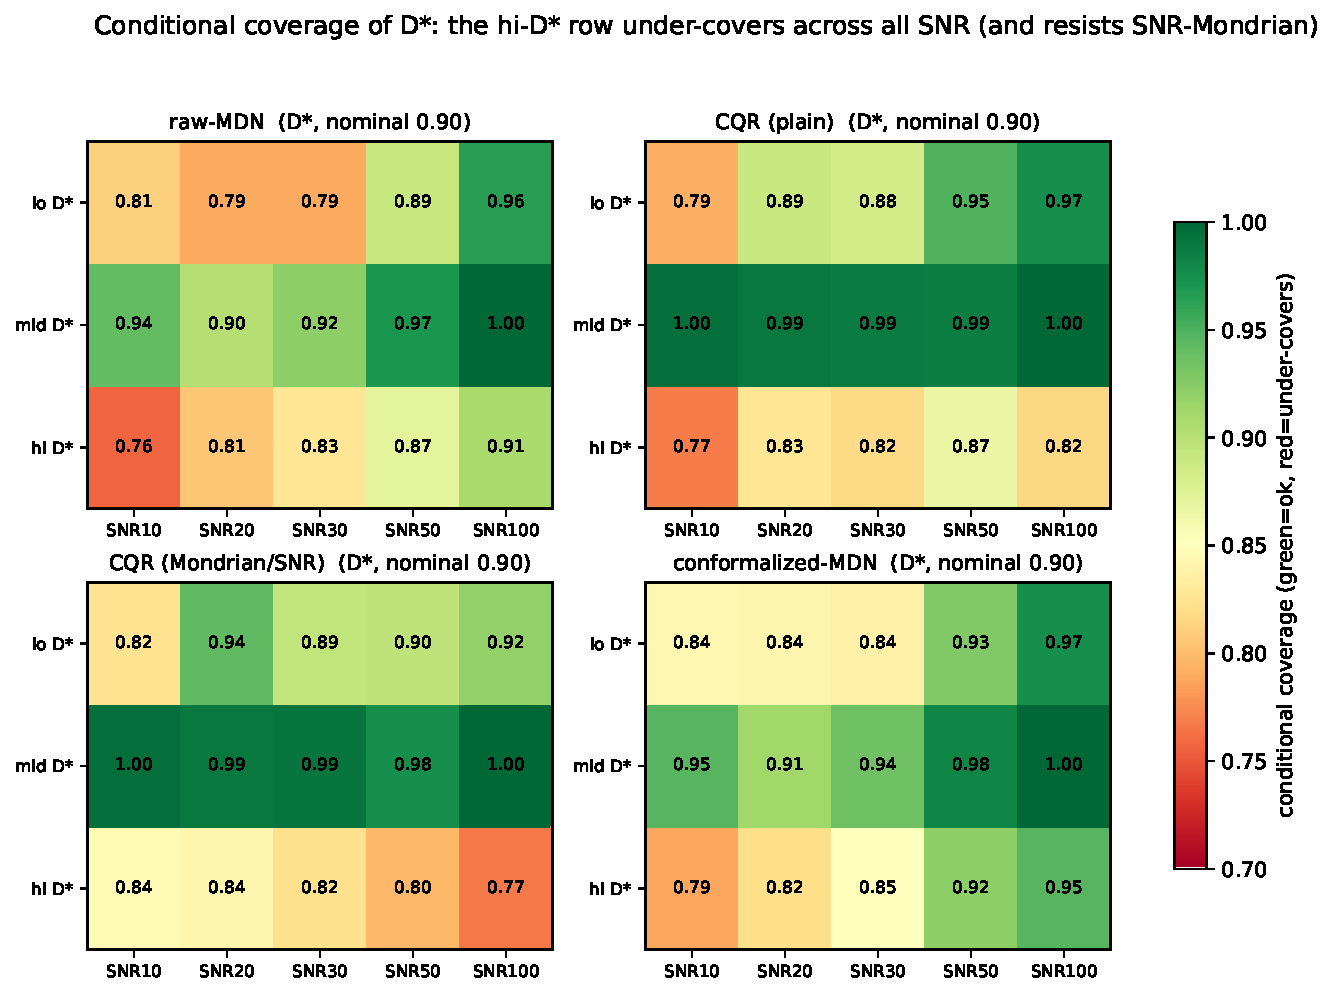
\includegraphics[width=0.72\linewidth]{figures/conditional_coverage_heatmap.pdf}
\caption{SNR $\times$ $\Dstar$-regime conditional coverage. The high-$\Dstar$ row
under-covers robustly at low-to-moderate SNR (recovering toward nominal only at the
highest SNR) and resists SNR-Mondrian.}
\label{fig:heatmap}
\end{figure}

\subsection{The high-$\Dstar$ gap is a latent-axis identifiability limit}
\label{sec:identifiability}
We attacked the high-$\Dstar$ gap with eleven \emph{label-free} conditioning
methods -- plug-in Mondrian by estimated $\hat{\Dstar}$, localized conformal on
observable features~\citep{guan2023}, and conditional conformal over an observable
basis~\citep{gibbs2023} -- none of which uses the true $\Dstar$
(Fig.~\ref{fig:attack}). \emph{None materially closes the gap.} The best label-free
method (MDN with localized conformal) reaches $0.874$\band{0.860}{0.899} marginal /
$0.807$\band{0.774}{0.845} worst-SNR, within sampling noise of the $0.786$ baseline.
The reason is structural, not
methodological:
\begin{itemize}
\item \textbf{Routing error.} A plug-in $\hat{\Dstar}$ misroutes $\sim33\%$
($[30,35]\%$ over 16 seeds) of true high-$\Dstar$ voxels to a lower-$\Dstar$
(smaller-radius) stratum -- least reliable exactly where it must route correctly.
Mondrian-by-$\hat{\Dstar}$ attains nominal coverage \emph{conditional on the observed
stratum} ($[0.90,0.89,0.90]$) yet craters on the \emph{true} high-$\Dstar$ tercile
($0.78$\band{0.76}{0.80}): it controls the observable, not the latent axis.
\item \textbf{The CRLB wall.} The CRLB on $\Dstar$ grows $\sim6\times$ from low to high
$\Dstar$ (an analytic, seed-invariant bound), and the ratio of median CRLB($\Dstar$)
to the tercile bin width rises $0.34\to0.67\to1.10$ across terciles (high-tercile band
$[1.02,1.15]$, Fig.~\ref{fig:crlb}). Where the CRLB \emph{exceeds} the bin width a
voxel's $\Dstar$ cannot be localized to its own tercile, so no observable can route it
to a wider-interval stratum; conformal width correctly tracks the per-voxel CRLB
(log--log $r=0.76$\band{0.72}{0.77}), so the intervals are honest, not broken.
\end{itemize}
\textbf{Verdict.} High-$\Dstar$ regime-conditional coverage is unrecoverable
label-free for two compounding reasons: the conditioning axis (true $\Dstar$ regime)
is latent and unidentifiable, so distribution-free conditional coverage on it is
impossible~\citep{barber2021limits} -- the operative barrier to coverage -- and,
separately, $\Dstar$ is poorly point-identified there (CRLB $\approx$ regime-bin
width), which is why even the point map is untrustworthy. We \emph{characterize} the
limit; we do not claim to solve it.

\begin{figure}[t]
\centering
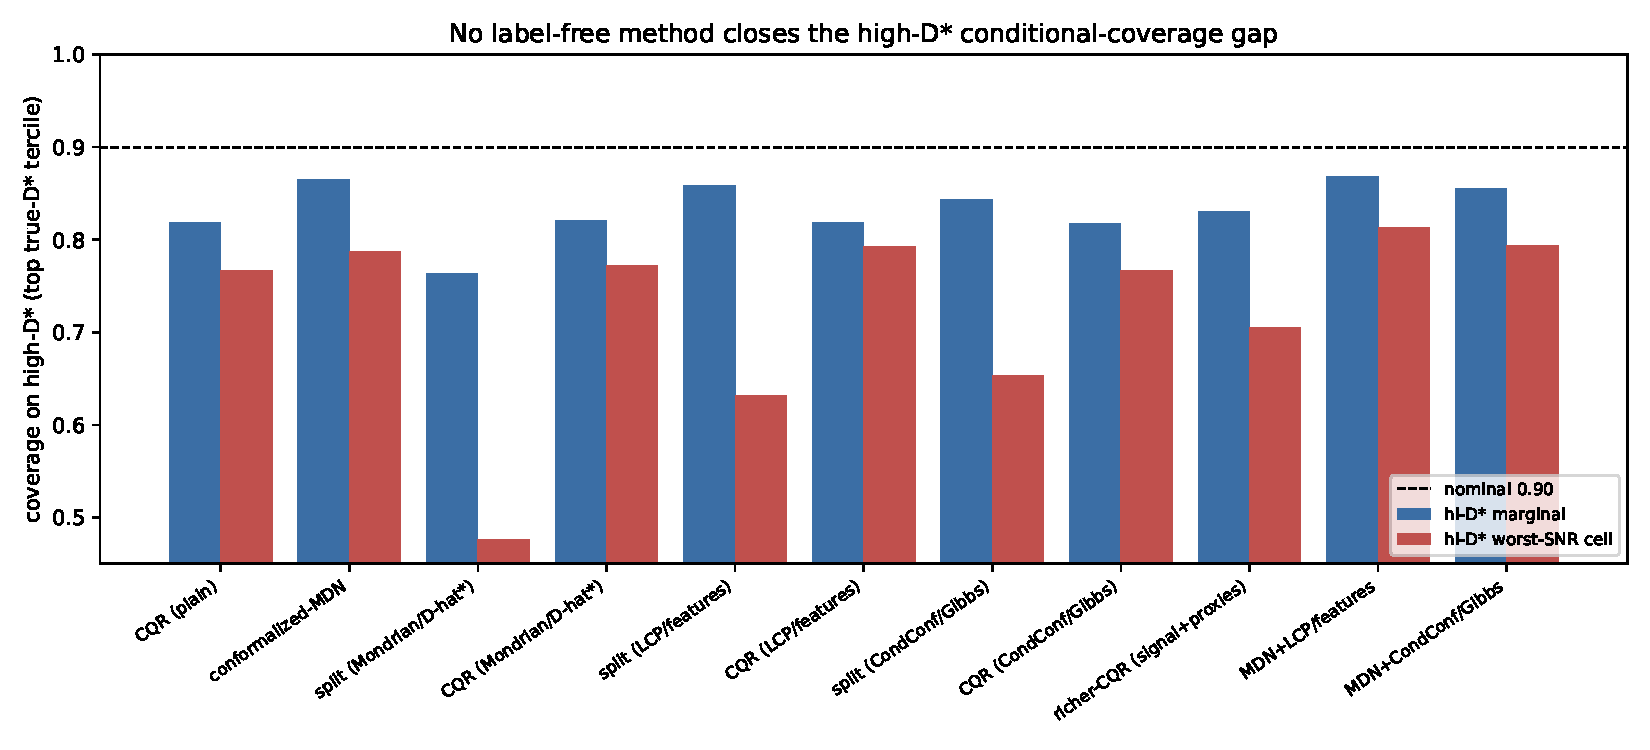
\includegraphics[width=0.82\linewidth]{figures/highdstar_attack.pdf}
\caption{High-$\Dstar$ coverage (marginal and worst-SNR cell) for eleven label-free
conditioning methods; every bar sits below the nominal $0.90$.}
\label{fig:attack}
\end{figure}

\begin{figure}[t]
\centering
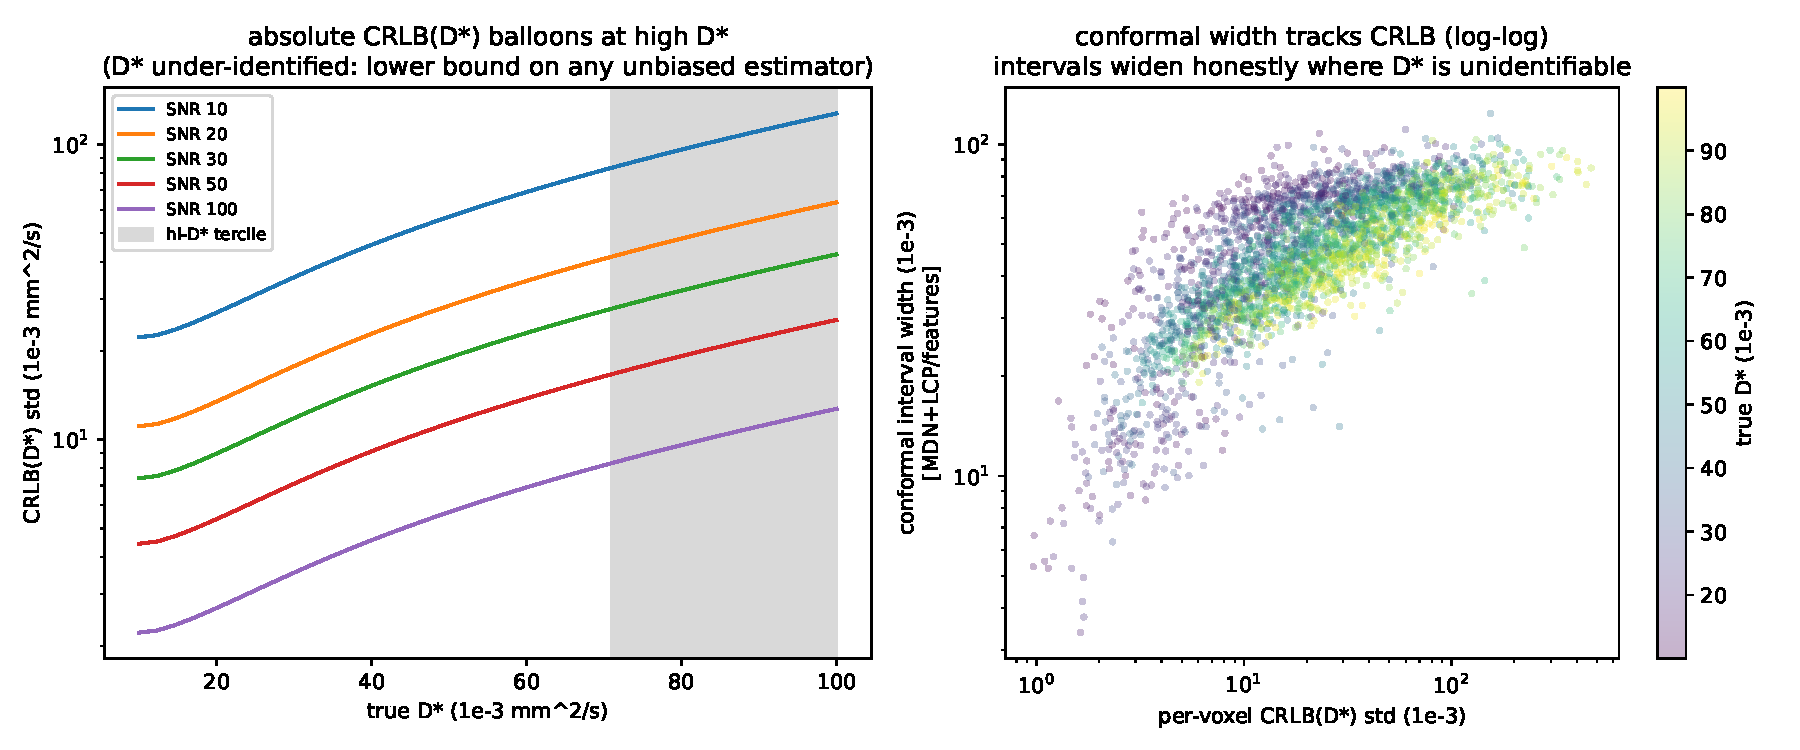
\includegraphics[width=0.92\linewidth]{figures/crlb_identifiability.pdf}
\caption{(Left) absolute CRLB($\Dstar$) balloons across the $\Dstar$ range per SNR
(high-$\Dstar$ tercile shaded). (Right) conformal width vs per-voxel CRLB
($r=0.76$): the intervals widen honestly where $\Dstar$ is under-identified.}
\label{fig:crlb}
\end{figure}

\subsection{Robustness under deliberate exchangeability breaks}
\label{sec:robustness}
We deploy one conformal predictor and one monitor, calibrated on the i.i.d.\ Rician
cohort, against four deliberate breaks; per-parameter naive-vs-weighted coverage and
the monitor verdict for each break are tabulated in Supporting Information
Table~\ref{tab:shift} (and Fig.~\ref{fig:shift}). Every break miscalibrates coverage:
the dangerous under-coverage reaches $\Dstar=0.508$\band{0.479}{0.543} under a
harder-tissue prior shift and the worst parameter $0.592$\band{0.557}{0.637} under a
low-SNR covariate shift. \emph{Weighted / nonexchangeable
conformal}~\citep{tibshirani2019,barber2023} recovers the covariate shifts (SNR
worst-parameter $0.592\to0.882$, all within $0.018$ of nominal; prior $\Dstar$
$0.508\to0.991$\band{0.974}{1.000}) but is honestly limited on tri-exponential
forward-model misspecification -- a shift in the conditional law $P(y\mid x)$ is not
repairable by an $x$-space likelihood ratio (weighting over-corrects $\Dstar$ to
$0.933$\band{0.924}{0.941}, a per-parameter spread of $0.033$). The label-free
monitor \textbf{fires on all four observable breaks before coverage fails}: in an
SNR-severity sweep it alarms at SNR $20$ (coverage still $0.866$) while coverage
first crosses the failure line at SNR $13$. Yet it is constitutively \emph{blind} to
the latent high-$\Dstar$ gap: on an in-distribution test the monitor is silent (AUC
$0.50$) and marginal $\Dstar$ coverage is nominal ($0.898$\band{0.880}{0.913}) while
the high-$\Dstar$ conditional coverage is $0.814$\band{0.787}{0.839} -- the same
observable-vs-hidden split that recurs across this work.


\subsection{Acquisition sensitivity: the wall is b-scheme-robust}
\label{sec:acquisition}
Does the high-$\Dstar$ wall move with the b-value scheme? We compare a clinical
($11$-value), a CRLB-optimal ($11$-value, greedy $\Dstar$-CRLB design), and a dense
($22$-value) scheme at fixed prior/SNR/seed; high-$\Dstar$ coverage and the
resolution ratio per scheme are in Supporting Information Table~\ref{tab:acq} and
Fig.~\ref{fig:acq}. The high-$\Dstar$ marginal coverage barely moves
($0.821\to0.835\to0.808$), and the resolution ratio CRLB($\Dstar$)/tercile-width
stays at or above unity: even a CRLB-optimal design only reaches $\sim$unity
($1.03$\band{0.97}{1.16}, down from the clinical $1.24$ and dense $1.11$). A
CRLB-optimal design lowers the ratio ($1.24\to1.03$) but does not remove the wall:
acquisition design \emph{shifts} the wall, it does not erase it -- a concrete,
honestly negative handoff to acquisition-aware experiment design.

\subsection{In-vivo: a qualitative demonstration, no coverage claim}
\label{sec:invivo}
In vivo there are no ground-truth parameters, so realized coverage is
\emph{unmeasurable} and the finite-sample guarantee is \emph{not asserted}. We
demonstrate the deployed pipeline qualitatively (Supporting Information
Fig.~\ref{fig:invivo}): the conformalized $\Dstar$ band widths are wide and
heavy-tailed ($10/50/90$th percentile $=47/64/79\times10^{-3}\unit{mm^2/s}$;
widest-to-narrowest decile ratio $1.7\times$), ballooning where the perfusion
compartment is under-identified -- the wall, now on signal. Pointed at the deployment
data with a synthetic calibration, the deployment monitor \textbf{fires} (AUC $0.84$):
synthetic$\to$deployment is itself a large exchangeability break, turning ``no ground
truth'' into an observable stop sign and giving the honest, label-free reason the
synthetic guarantee must not be transferred in vivo without re-calibration on matched
labeled data, which in vivo does not exist.


\subsection{Real in-vivo data: the same pipeline, the monitor fires on transfer}
\label{sec:invivo-real}
We additionally run the as-deployed pipeline on real multi-$b$ in-vivo DWI from the
public ACRIN-6698 / I-SPY2 Breast DWI collection (The Cancer Imaging Archive;
CC-BY-4.0)~\cite{acrin6698,clark2013tcia}, retrieved on demand. This is a 4-$b$ ADC
protocol ($b=\{0,100,600,800\}\unit{s/mm^2}$), \emph{not} IVIM-optimized, with no
ground-truth IVIM parameters, so it supports only qualitative pipeline/monitor
behavior and makes \textbf{no in-vivo coverage claim}. A predictor trained on the
synthetic 22-value scheme cannot ingest a 4-$b$ signal and interpolation would
fabricate unacquired $b$-values, so we keep the deployment \emph{monitor} as-deployed
(its observable features are $b$-independent) and re-fit only the CQR band at the real
4-$b$ scheme; the resulting bands are qualitative, not coverage intervals.

The real $b{=}0$ breast DWI, the plug-in $\hat{\Dstar}$ map, and the per-voxel
conformal $\Dstar$ band-width (uncertainty) map with the whole-tumor ROI are shown in
Supporting Information Figure~\ref{fig:invivo-maps}; the uncertainty map is spatially
heterogeneous and widens where the perfusion compartment is under-identified, the wall
now visible on real tissue.

On $4000$ foreground voxels the as-deployed monitor \textbf{fires} (AUC $0.97$) and
the $\Dstar$ band stays wide ($10/50/90$th percentile
$=64/79/86\times10^{-3}\unit{mm^2/s}$; Fig.~\ref{fig:invivo-real}). The firing is
carried entirely by the $b$-independent Mahalanobis family; the residual family is
silent because a 4-$b$ acquisition exactly-determines the four-parameter fit,
collapsing the residual norm to zero -- so the monitor has \emph{not} half-failed but
localized the break to the feature distribution. The sparse-protocol-plus-real-tissue
gap is a large exchangeability break, which is exactly why the synthetic guarantee
\emph{correctly refuses} to transfer.

\paragraph{Test--retest repeatability.}
ACRIN-6698 includes a same-day test--retest arm -- two coffee-break repeat DWI exams
in a single visit (\texttt{TrT0}/\texttt{TrT1}; this genuine same-visit arm supersedes
an earlier $n{=}11$ pairing that had inadvertently matched \emph{longitudinal}
timepoints months apart). Across $n{=}76$ tumors we ask, label-free, whether the
conformal interval width \emph{tracks} the scan--rescan variability of the plug-in
estimate (region-level over the whole-tumor ROI; the repeats are unregistered, so not
a per-voxel statement). The wall makes a directional prediction we fix before looking:
width should track measured scan--rescan repeatability for the well-identified $D$ and
weakly or not at all for $\Dstar$, whose regime the data cannot resolve -- a positive
$\Dstar$ association would count against the wall. For $D$, the conformal $D$-width is
associated with the measured scan--rescan $|\Delta\mathrm{ADC}|$ (Spearman $r=+0.60$,
$p<0.001$, 95\% CI $[0.42,0.72]$ by BCa bootstrap): the interval \emph{widens where
the real measurement is least repeatable}. At $n{=}76$ this is now \textbf{robust} (CI
excludes zero, versus the wide interval at $n{=}11$) and stable across field strength
(1.5\,T $r{=}{+}0.58$, $n{=}49$; 3.0\,T $r{=}{+}0.50$, $n{=}27$) and pretreatment-only
($r{=}{+}0.61$, $n{=}65$). For $\Dstar$ the association is not significant
($r=-0.17$, $p=0.13$, 95\% CI $[-0.39,0.05]$ spanning zero), matching the pre-stated
prediction. This is a repeatability-tracking check, \emph{not} validation, accuracy,
calibration, or coverage.

\begin{figure}[t]
\centering
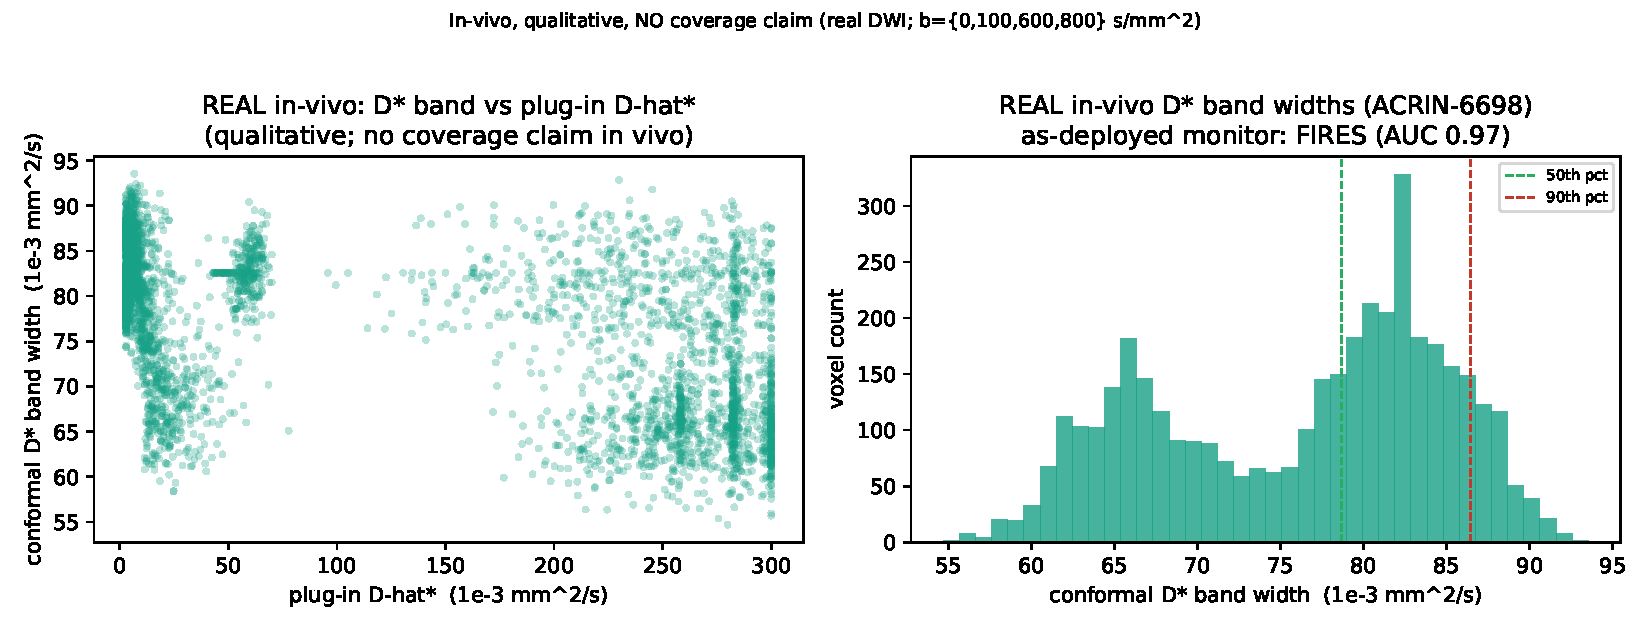
\includegraphics[width=0.92\linewidth]{figures/invivo_real_demo.pdf}\\[2pt]
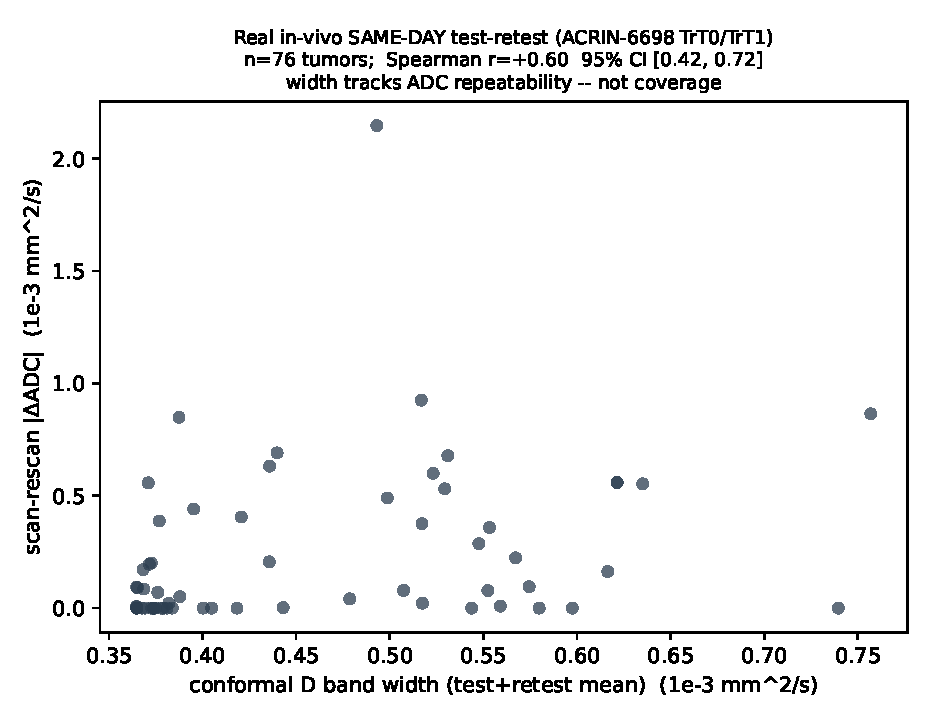
\includegraphics[width=0.55\linewidth]{figures/invivo_real_retest.pdf}
\caption{Real in-vivo data (ACRIN-6698 / I-SPY2 Breast DWI; qualitative, no coverage
claim). (Top left) the re-fit conformal $\Dstar$ band vs the plug-in $\hat{\Dstar}$;
(top right) the $\Dstar$ band-width distribution and the as-deployed monitor verdict
(fires, AUC $0.97$, via the $b$-independent Mahalanobis family). (Bottom)
test--retest: the conformal $D$-width vs the measured scan--rescan ADC variability
across $n{=}76$ same-day-repeat tumors (Spearman $r=+0.60$, 95\% CI $[0.42,0.72]$;
robust, repeatability-tracking only---not validation or coverage).}
\label{fig:invivo-real}
\end{figure}

\subsection{External-phantom replication on the OSIPI IVIM reference}
\label{sec:osipi}
Every coverage number above is computed on \emph{our} labeled synthetic cohort. To
neutralise the ``validated only on the authors' own forward model'' concern, we
replicate the coverage results and the high-$\Dstar$ wall against an \textbf{external,
community-standard \emph{synthetic} reference}: the OSIPI (ISMRM Open Science
Initiative for Perfusion Imaging) TF2.4 IVIM digital reference object (DRO), $5000$
voxels with ground-truth $(D,\Dstar,f)$ \emph{we did not generate}~\citep{osipi_ivim}
(Zenodo \texttt{doi:10.5281/zenodo.14605039}, CC-BY-4.0; fetched on demand). This is
an \emph{independent synthetic} reference, \textbf{not} in vivo, so no in-vivo
coverage claim is made. The bi-exponential signal model is the field's consensus and
shared by construction; what is external is the ground-truth \emph{parameter
distribution}, genuinely shifted from ours: the OSIPI true $\Dstar$ spans
$\sim\!0.05$--$0.20\,\mathrm{mm^2/s}$, above our calibration prior ($0.01$--$0.10$),
so transferring our calibration onto it is a real out-of-distribution test. All
numbers are across-seed means with $[5,95]$ bands over $16$ seeds; nominal coverage
is $0.90$.

We evaluate two regimes -- \emph{controlled} (OSIPI ground truth re-synthesised at
\emph{our} 22-$b$ acquisition and SNR grid, so only the parameter distribution is
swapped) and \emph{native} (the DRO's own pre-noised signals at its native sparse
7-$b$ scheme) -- each under \emph{naive transfer} (calibrate on our cohort, test on
OSIPI) and \emph{recalibrated} (split the OSIPI DRO and calibrate within its
distribution). The full marginal and top-$\Dstar$-tercile coverage grid is in
Supporting Information Table~\ref{tab:osipi}; Fig.~\ref{fig:osipi} plots it with the
wall metric.

\paragraph{Naive transfer breaks, and the monitor says so.} Transferring our
synthetic calibration onto the OSIPI ground truth breaks marginal coverage
(controlled $\Dstar$ $0.304$\band{0.285}{0.315}, $D$ $0.597$\band{0.567}{0.621}),
exactly as exchangeability theory predicts for a real distribution shift, and the
label-free deployment monitor \emph{fires on every one of the $16$ seeds}
(Mahalanobis AUC $0.737$\band{0.726}{0.750}, controlled): the shift is observable, so
the monitor correctly refuses the transfer (cf.\ \S\ref{sec:invivo-real}).

\paragraph{Recalibrated coverage holds, yet the high-$\Dstar$ wall replicates.}
Splitting the OSIPI DRO and recalibrating within its own distribution restores
marginal coverage to nominal for all three parameters ($D$ $0.899$\band{0.881}{0.913},
$\Dstar$ $0.905$\band{0.889}{0.921}, $f$ $0.904$\band{0.892}{0.919}; native nearly
identical) -- the finite-sample guarantee transfers cleanly to a forward model and
prior we did not author. Yet coverage conditional on the true $\Dstar$ tercile still
craters in the high-$\Dstar$ regime ($0.823$\band{0.786}{0.853} controlled,
$0.831$\band{0.798}{0.869} native) while the low-$\Dstar$ tercile sits at nominal
($0.899$\band{0.859}{0.931}). On the OSIPI ground truth at our acquisition the
CRLB$(\Dstar)$/tercile-width ratio rises $0.46\!\to\!0.86\!\to\!1.53$
(\band{1.407}{1.753} at high $\Dstar$) with the absolute CRLB growing
$3.5\times$\band{3.1}{4.0} -- the same wall as Fig.~\ref{fig:crlb}, on a reference we
did not build. The regime also dissociates the two mechanisms: in the native
high-SNR setting the CRLB ratio stays below $1$ yet the conditional gap persists, so
the coverage failure survives where the CRLB does \emph{not} exceed the bin width --
driven by conditioning on a latent axis the data do not
identify~\citep{barber2021limits}, not by CRLB magnitude -- strong evidence the wall
is information-theoretic, intrinsic to the perfusion-estimation problem rather than
our forward model or prior.

\begin{figure}[t]
\centering

\includegraphics[width=\linewidth]{figures/osipi_coverage.pdf}
\caption{OSIPI external \emph{synthetic} reference (DRO; not in vivo, no in-vivo
coverage claim). (A) Marginal coverage vs nominal: naive transfer of our synthetic
calibration breaks, recalibrating within the OSIPI distribution restores it. (B)
Coverage conditional on the true $\Dstar$ tercile: the high-$\Dstar$ gap persists
even after recalibration. (C) The identifiability wall on OSIPI ground truth --
CRLB$(\Dstar)$ exceeds the high-$\Dstar$ tercile width. The naive-transfer monitor
fires (AUC $0.74$), so the break is flagged.}
\label{fig:osipi}
\end{figure}

\subsection{Point accuracy does not buy conditional coverage: a deliberately
biased estimator}
\label{sec:dissociation-shrinkage}
A natural objection to the identifiability reading is that the unbiased baselines
merely leave precision on the table: a \emph{biased} prior-shrinkage Bayesian fit was
historically the one IVIM estimator that kept $\Dstar$ variance under control, and a
biased estimator can legitimately sit below the \emph{unbiased} Cram\'er--Rao
bound~\citep{gurneychampion2018}. If the high-$\Dstar$ wall were a point-precision
artifact, such an estimator should breach it. We pushed a deliberately biased,
label-free shrinkage prior (a fixed log-normal $\Dstar$/$f$ prior with the
NLLS-residual noise scale, using no labels) through the same conditional-coverage
machinery (Table~\ref{tab:dissociation}).

The prior behaves as a shrinkage prior should: it lowers $\Dstar$ point RMSE in the
low tercile ($15.1$\band{14.7}{15.6} vs.\ the unbiased MCMC's
$17.8$\band{17.2}{18.5}, in $10^{-3}$\,mm$^2$/s) by trading variance for a
centre-pulling bias. But in the deciding high-$\Dstar$ tercile that bias dominates:
point RMSE does \emph{not} improve ($24.6$\band{24.1}{25.3} vs.\
$20.5$\band{19.9}{21.1}), carried by a large negative bias
($-18.8$\band{-19.2}{-18.3} vs.\ $-14.2$\band{-14.5}{-13.7}). Crucially, high-$\Dstar$
regime-conditional coverage does not rise: the conformalized marginal
$0.827$\band{0.801}{0.845} and worst-SNR cell $0.721$\band{0.663}{0.765} sit at or
below the unbiased arms ($0.889$\band{0.872}{0.903} / $0.857$\band{0.826}{0.875} for
MCMC), nowhere near nominal $0.90$. Two pre-registered sanity gates exclude artifacts:
the shrinkage interval does \emph{not} collapse (median high-$\Dstar$ width
$55.0$\band{53.6}{56.6} vs.\ comparator $47.9$, in $10^{-3}$; $1.15\times$), and the
estimator still misroutes $34$\band{32}{36}\% of true-high-$\Dstar$ voxels (the NLLS
plug-in misroutes $\sim33\%$), so any coverage change would arise \emph{despite}
routing, not by repairing it. Trading variance for bias buys point precision in the
identified terciles but not conditional coverage where the conditioning axis is
latent: the barrier is information, not point precision. The argument is
mechanism-level -- any centre-pulling bias dominates in the high-$\Dstar$ tercile, so
it brackets the historically $\Dstar$-stabilizing prior-shrinkage Bayesian
fit~\citep{gurneychampion2018} rather than one prior choice, while remaining a
statement about the label-free methods we tested.

\begin{table}[t]
\centering
\caption{Point-accuracy / conditional-coverage \emph{dissociation} for a
deliberately biased shrinkage prior. RMSE and bias in $10^{-3}$\,mm$^2$/s; coverage
of the conformalized $\Dstar$ band (nominal $0.90$). Across-seed means with 16-seed
$[5,95]$ bands. From \texttt{results/multiseed\_report.txt} /
\texttt{results/dissociation\_report.txt}.}
\label{tab:dissociation}
\small
\begin{tabular}{lcccc}
\toprule
arm & hi-$\Dstar$ RMSE & hi-$\Dstar$ bias & hi-$\Dstar$ marginal & hi-$\Dstar$ worst-SNR \\
\midrule
Bayesian-shrinkage & 24.6\band{24.1}{25.3} & $-18.8$\band{-19.2}{-18.3} & 0.827\band{0.801}{0.845} & 0.721\band{0.663}{0.765} \\
Bayesian-MCMC      & \textbf{20.5}\band{19.9}{21.1} & $-14.2$\band{-14.5}{-13.7} & \textbf{0.889}\band{0.872}{0.903} & \textbf{0.857}\band{0.826}{0.875} \\
conformalized-MDN  & 20.3\band{19.6}{21.0} & $-13.4$\band{-14.2}{-12.8} & 0.867\band{0.853}{0.884} & 0.784\band{0.742}{0.819} \\
\bottomrule
\end{tabular}
\end{table}

\subsection{The wall replicates under a non-bi-exponential generator}
\label{sec:altmodel}
The external-phantom replication still draws its ground truth from a bi-exponential
model. To test whether the high-$\Dstar$ wall is an artifact of Eq.~\eqref{eq:ivim}
itself, we regenerate the cohort from a genuinely \emph{non}-bi-exponential mechanism:
a gamma velocity-dispersion perfusion process (coefficient of variation $0.5$, shape
$k=4$) whose signal is \emph{not} a realization of Eq.~\eqref{eq:ivim}. Because such a
signal has no single ``true''
$\Dstar$, we report the effective pseudo-diffusion $\Dstar_{\mathrm{eff}}$ on two
axes: a primary, non-circular axis (A), the analytic perfusion log-slope (gamma mean,
defined without a bi-exponential fit), and a corroborating axis (B), the best-fit
bi-exponential $\Dstar$, reported only to confirm the two definitions agree.
Calibration and recalibration use the OSIPI within-distribution harness
(Sec.~\ref{sec:osipi}).

After recalibrating \emph{within} the dispersion distribution, marginal coverage is
restored ($\Dstar_{\mathrm{eff}}$ marginal $0.898$\band{0.880}{0.917} on axis A),
yet the high-$\Dstar_{\mathrm{eff}}$ tercile-conditional coverage stays well below
nominal on both axes -- $0.796$\band{0.748}{0.854} (A) and $0.800$\band{0.756}{0.845}
(B) (Fig.~\ref{fig:altmodel}A), a gap of $\sim0.10$ the bi-exponential CRLB cannot
have caused because the generator is not bi-exponential. The wall is therefore a
property of the perfusion-estimation problem more broadly: it survives a generator
Eq.~\eqref{eq:ivim} does not even contain. A second dispersion kernel (log-normal,
same CV) reproduces it (high-$\Dstar_{\mathrm{eff}}$ $0.797$\band{0.747}{0.847}), so
it is not gamma-specific, and a continuity gate confirms soundness: at zero dispersion
the generator reduces to the bi-exponential cohort exactly (max
$|S_{\mathrm{disp}}(\mathrm{CV}{=}0)-S_{\mathrm{biexp}}|=0.00\mathrm{e}{+}00$), with
recalibrated high-$\Dstar$ coverage there ($0.798$\band{0.750}{0.842}) landing on the
bi-exponential wall. Consistent with the observable-vs-latent reading, this
forward-model misspecification is largely a \emph{hidden} channel: the naive-transfer
monitor barely separates the dispersion cohort from the bi-exponential calibration
(AUC $0.501$\band{0.481}{0.519}, at chance).

\subsection{The off-model validity envelope}
\label{sec:envelope}
The tri-exponential stress in Sec.~\ref{sec:robustness} is a single off-model probe.
We replace it with a \emph{validity envelope}: holding the deployed,
bi-exponential-calibrated predictor fixed, we sweep three independent deviation
families -- velocity dispersion (CV up to $0.8$), a tri-exponential third compartment
(weight up to $0.4$), and a stretched-exponential signal ($|1-\beta|$ up to $0.6$) --
tracing coverage degradation and monitor drift (Fig.~\ref{fig:altmodel}B,C). Marginal
coverage degrades gracefully and monotonically: by the largest deviation, $\Dstar$
coverage falls to $0.769$\band{0.736}{0.788} (tri-exponential) and
$0.770$\band{0.749}{0.793} (stretched), and perfusion-fraction coverage to
$0.791$\band{0.767}{0.815} (dispersion), while at zero deviation it recovers to
nominal ($\Dstar$ $0.903$\band{0.880}{0.918}). The monitor's discrimination is real
but weak and family-dependent -- AUC rises with deviation for the tri-exponential
family ($0.532$\band{0.515}{0.548} at the largest step) yet stays near chance for
pure velocity dispersion -- so off-model misspecification is only partly observable,
reinforcing that some forward-model breaks are hidden channels. The single
tri-exponential probe thus generalizes to a characterized envelope.

\begin{figure}[t]
\centering
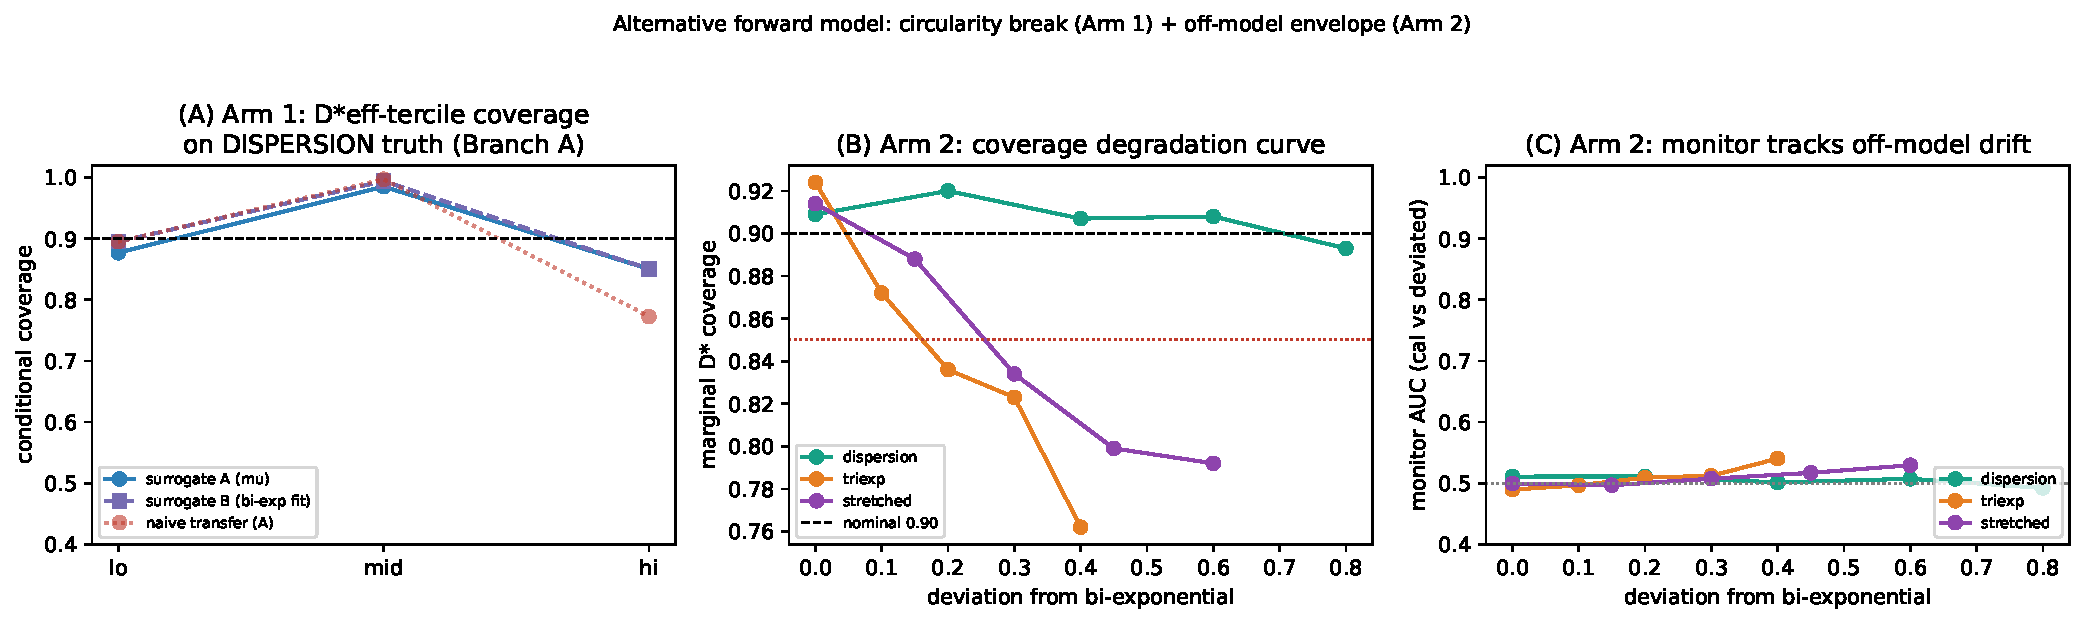
\includegraphics[width=\linewidth]{figures/altmodel.pdf}
\caption{Alternative forward model. (A) Arm~1 -- $\Dstar_{\mathrm{eff}}$-tercile
conditional coverage when the ground truth is a non-bi-exponential velocity-dispersion
process: after within-distribution recalibration the high-$\Dstar_{\mathrm{eff}}$
gap persists on both surrogate axes (primary gamma mean A, corroborating bi-exp-fit B), while naive
transfer breaks. (B) Arm~2 -- marginal $\Dstar$ coverage degrades monotonically as
the forward model deviates from bi-exponential across three families, recovering to
nominal at zero deviation. (C) Arm~2 -- the deployment monitor's AUC vs.\ deviation:
discrimination of off-model drift is weak and family-dependent. Across-seed means
(16 seeds); from \texttt{results/altmodel\_report.txt}.}
\label{fig:altmodel}
\end{figure}

\subsection{A clinically realistic cohort: correlated prior and measurement nuisance}
\label{sec:realism}
The cohort so far draws $(D,\Dstar,f)$ uniformly over published ranges with clean
Rician noise. As a capstone we replace both idealizations at once: a clinically
realistic \emph{joint} prior -- correlated, right-skewed marginals (log-normal
$D,\Dstar$; logit-normal $f$) with a within-subject $\Dstar$ coefficient of variation
in the published $50$--$110\%$ band, \emph{shaped to approximate} (not fitted to)
abdominal IVIM cohorts~\citep{gurneychampion2018,kaandorp2021,barbieri2020} as
documented design constants (Supporting Information Table~\ref{tab:realism-prior}) --
and a measurement-level nuisance layer on the signal under a single magnitude scalar
$\eta$: partial-volume mixing of a free-fluid compartment, bulk-motion phase, and
non-Rician (multi-coil noncentral-$\chi$) noise. This is still synthetic and makes no
in-vivo coverage claim; a continuity gate confirms it reduces to the existing cohort
exactly at the uniform prior with $\eta=0$ (max $|\cdot|=0.00\mathrm{e}{+}00$). Because
a skewed prior moves the tercile boundaries, we report the high-$\Dstar$ regime on two
stratifications -- \emph{fixed} physical boundaries inherited from the uniform cohort
(primary, so ``high $\Dstar$'' denotes the same physical regime across priors) and
per-distribution quantiles (secondary) -- with the clinical prevalence of the fixed
bin reported so a rare regime is never mistaken for a vanished wall.

Under the realistic prior with clean acquisition (Arm~A), recalibrating
\emph{within} the distribution restores marginal coverage to nominal ($D/\Dstar/f =
0.903$\band{0.896}{0.913}, $0.900$\band{0.884}{0.917}, $0.898$\band{0.885}{0.912}),
while naive transfer of the uniform-calibrated predictor breaks ($\Dstar$ marginal
$0.767$\band{0.735}{0.805}). The high-$\Dstar$ wall persists in \emph{both}
stratifications -- fixed-edge tercile coverage $0.533$\band{0.480}{0.594} and
per-distribution $0.786$\band{0.749}{0.823}, against nominal $0.90$ -- with the
fixed-edge CRLB-to-bin-width ratio reaching $0.895$\band{0.849}{0.961}
(Fig.~\ref{fig:realism}A,B); as in the shrinkage dissociation
(Sec.~\ref{sec:dissociation-shrinkage}), a sub-unity ratio coexisting with a large gap
is expected, since the ratio bounds \emph{point} precision whereas the gap is a
\emph{conditional-coverage} failure on a latent axis. The severest under-coverage
concentrates in a clinically \emph{rare} high-$\Dstar$ tail (fixed prevalence
$0.049$\band{0.044}{0.056}), entangling bin rarity (few high-$\Dstar$ calibration
examples for the single global offset) with the wall itself. A calibration-size
control separates them: up-sampling the fixed high-$\Dstar$ \emph{calibration} count
to the uniform-prior level ($\sim\!73\to504$ voxels from the realistic generator -- a
fidelity gate confirms they match the realistic, not uniform, law), with train, test
and prior fixed, lifts coverage from $0.533$ only to $0.661$\band{0.580}{0.721},
closing $\approx\!47\%$ of
the way to the uniform-prior anchor $0.807$\band{0.774}{0.831} and never reaching it
($\le0.72$ in every seed; Fig.~\ref{fig:realism}D). Rare-bin sparsity thus accounts
for roughly half the fixed-edge deficit; the remainder is a genuine wall that survives
count-matching. The regime's rarity does not make it low-stakes -- a high-$\Dstar$
voxel is often the salient finding (brisk lesion perfusion). The realistic prior is a
within-support covariate shift, so the monitor does not flag it (naive-transfer AUC
$0.480$\band{0.470}{0.494}, at chance); recalibration, not monitoring, restores
coverage.

Holding the deployed predictor fixed and sweeping the nuisance magnitude (Arm~B),
marginal coverage degrades monotonically: $D$ coverage falls from
$0.903$\band{0.889}{0.912} at $\eta=0$ to $0.570$\band{0.548}{0.589} at $\eta=1$,
while the already-wide $\Dstar$ interval stays near nominal
($0.899$\band{0.888}{0.911}) and recalibrating restores it ($\Dstar$
$0.899$\band{0.886}{0.914} at $\eta=1$). This $\Dstar$ stability reflects interval
\emph{width}, not robust identification: the band is already wide enough to absorb the
nuisance, so flat $\Dstar$ coverage is the characterized-but-unresolved wall showing
through. This nuisance is no more observable than signal-model drift -- the monitor's
AUC stays at chance ($0.493$\band{0.482}{0.507} at $\eta=1$, cf.\ the off-model
envelope's $\le0.53$) -- so a measurement nuisance that substantially breaks coverage
is a largely \emph{silent} channel, again locating the safeguard in recalibration.

\begin{figure}[t]
\centering
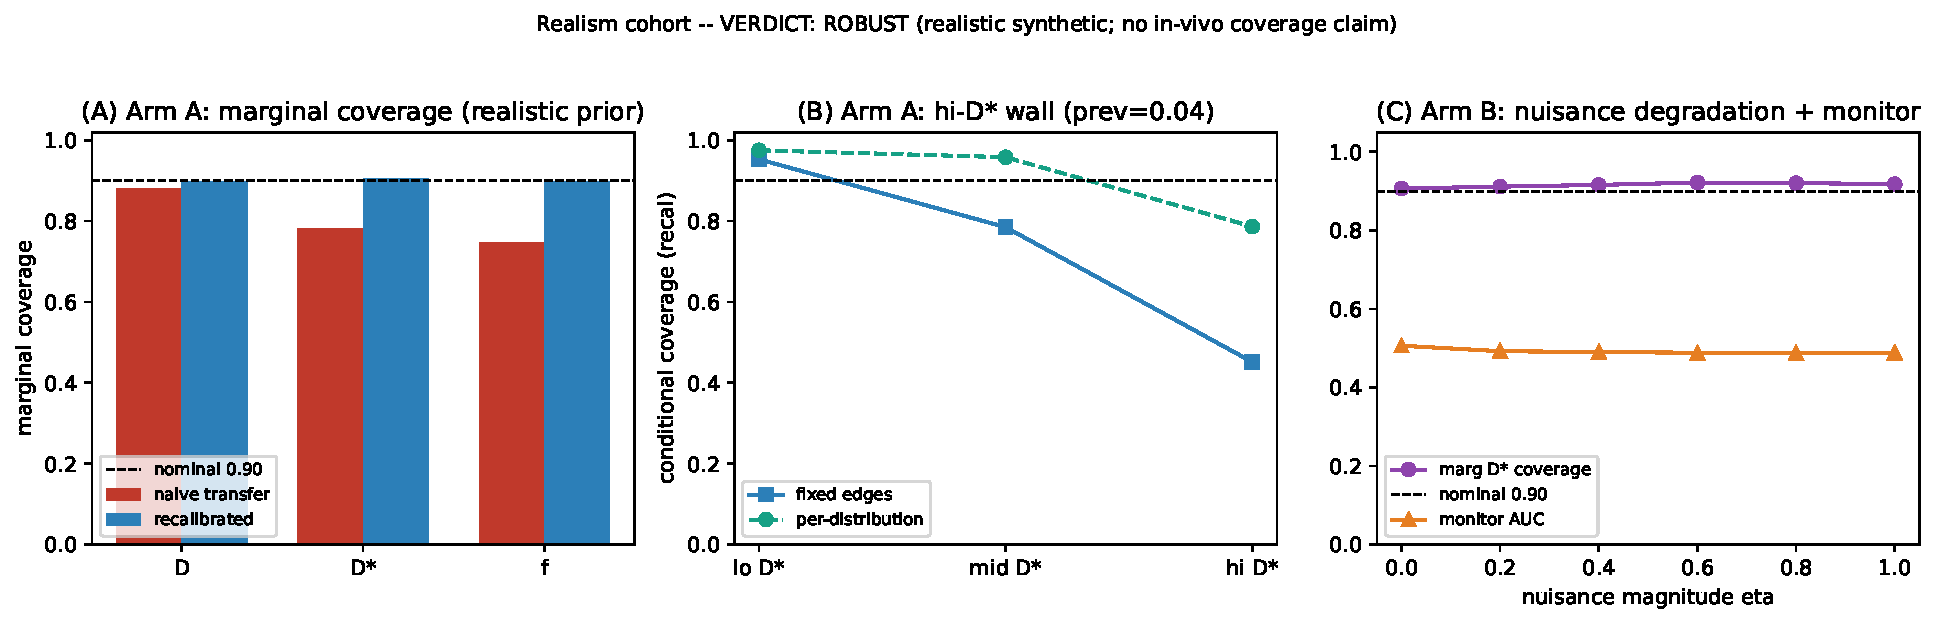
\includegraphics[width=\linewidth]{figures/realism_cohort.pdf}
\caption{Realism cohort (realistic synthetic; no in-vivo coverage claim).
(A)~Arm~A -- marginal coverage under a realistic correlated/skewed prior: naive
transfer of the uniform-calibrated predictor breaks, within-distribution
recalibration restores nominal coverage. (B)~Arm~A -- recalibrated high-$\Dstar$
tercile coverage on fixed physical boundaries vs.\ per-distribution quantiles; the
wall persists in both, concentrated in a clinically rare high-$\Dstar$ tail (fixed
prevalence $\approx0.05$). (C)~Arm~B -- the measurement-nuisance envelope: marginal
$D$ coverage degrades with the nuisance magnitude (the wider $\Dstar$ interval is
held) while the deployment monitor's AUC stays at chance, a silent channel.
(D)~NF1 calibration-size control: fixed-edge high-$\Dstar$ recalibrated coverage
under native vs.\ count-matched calibration (hi-$\Dstar$ calibration count
$73\to504$), against the uniform-prior anchor; only $\approx47\%$ of the
native$\to$uniform gap is closed by count-matching, isolating a residual wall.
Seed-\texttt{20260613} panel (across-seed [5,95] bands quoted in text); from
\texttt{results/realism\_report.txt}.}
\label{fig:realism}
\end{figure}

\section{Discussion}
The thread connecting these results is an \emph{observable-vs-latent} distinction.
Conformal prediction guarantees \emph{marginal} coverage and, with weighting or
stratification on \emph{observable} quantities (SNR, signal features, density ratios),
can recover coverage conditional on those observables; what it cannot
label-free-guarantee is coverage conditional on a \emph{latent} axis the data do not
identify. In IVIM that axis is the true $\Dstar$ in its ill-posed regime: the Fisher
information collapses, the CRLB exceeds the bin width, and no observable proxy --
including the plug-in $\hat{\Dstar}$ -- recovers the regime. This is why an observable
monitor catches every \emph{distribution} shift but is blind to the
\emph{within-distribution} high-$\Dstar$ gap. Four independent stresses corroborate
that this split is information, not an artifact of our estimator or generator: a
biased shrinkage prior buys $\Dstar$ point precision but not high-$\Dstar$ conditional
coverage (Sec.~\ref{sec:dissociation-shrinkage}); the gap replicates under a
non-bi-exponential velocity-dispersion generator, itself a hidden channel
(Sec.~\ref{sec:altmodel}); the off-model envelope degrades gracefully with a recovered
bi-exponential origin (Sec.~\ref{sec:envelope}); and the wall persists under a
clinically realistic correlated, skewed prior with measurement nuisance, concentrated
in a rare high-$\Dstar$ tail with the nuisance a silent channel
(Sec.~\ref{sec:realism}).

The same wall appears in adjacent label-free problems: deployment-validity monitoring
is provably blind to shifts that leave observable statistics unchanged (a ``hidden
channel''), and the absence of in-vivo ground truth forecloses any direct coverage
check on real data. We read these not as failures of conformal prediction -- whose
guarantee is exactly as advertised -- but as the IVIM instance of a known
boundary~\citep{barber2021limits}: distribution-free tools deliver everything the data
identify and nothing they do not. The finite-sample guarantee is a property of the
synthetic calibration and transfers in vivo only under an exchangeability assumption
that cannot be verified where no ground truth exists; it is not an in-vivo coverage
claim. What the method adds over the existing IVIM repeatability literature is
mechanistic and operational: (i) conformalizing a strong model-based base gives the
sharpest valid intervals on synthetic data; (ii) an observable monitor guards
exchangeability at deployment while remaining blind to the latent high-$\Dstar$ gap by
construction; and (iii) the high-$\Dstar$ compartment is reported as
characterized-but-unresolved, with a per-voxel reason -- the identifiability wall --
rather than a trusted point map.

\paragraph{What this means in practice.}
For a clinician or pipeline operator, the result is a triage rule, not a counsel of
despair. The tissue-diffusion compartment $D$ is the well-identified one: it carries
the finite-sample guarantee on the synthetic cohort and in real data its interval
width tracks measured scan--rescan repeatability (Sec.~\ref{sec:invivo-real}), so it
is the compartment to trust. The high-$\Dstar$ pseudo-diffusion map should instead be
read as \emph{characterized-but-unresolved}: its wide, honest interval is not a defect
but the correct signal that the data do not localize the parameter, with the per-voxel
CRLB supplying the reason. The deployment monitor turns the absence of in-vivo ground
truth into an observable stop sign, firing on exactly the transfers where the
synthetic guarantee must not be assumed. The contribution is operational: it tells the
user which compartment to trust and why to distrust the rest, rather than promising a
new biomarker.

\subsection{Limitations}
Our coverage results are \emph{synthetic-primary} by necessity: conformal calibration
needs labels that in-vivo IVIM lacks, so the guarantee is established on a forward
model we control and the in-vivo component is explicitly qualitative. This is a
structural impossibility, not a removable study limitation: because in-vivo IVIM
admits no ground-truth $(D,\Dstar,f)$, realized coverage is unmeasurable in vivo in
principle, so a distribution-free guarantee can only be synthetic-established and then
transported under an explicitly monitored exchangeability assumption -- precisely what
Sec.~\ref{sec:invivo-real} exercises. The base cohort uses uniform priors and Rician
noise; we address the heterogeneity of real tissue with a capstone realism cohort
(Sec.~\ref{sec:realism}: correlated skewed prior plus measurement nuisance), where the
marginal guarantee returns on recalibration and the high-$\Dstar$ wall persists. The
off-model behavior is likewise characterized rather than probed at a single point
(Secs.~\ref{sec:altmodel},~\ref{sec:envelope}), but these remain schematic deviations
and a still-synthetic cohort, not a validated tissue model, and the in-vivo
unverifiability above is unchanged by them. The CRLB diagnostic uses the high-SNR
Gaussian approximation to Rician noise; the qualitative under-identification of
$\Dstar$ is noise-model-independent (the $\Dstar$ Jacobian column vanishes as $\Dstar$
grows), but absolute bound values at SNR $\lesssim10$ would shift under an exact Rician
treatment. Finally, all coverage guarantees assume exchangeability of calibration and
deployment data; the monitor quantifies, but cannot by itself repair, departures from
it.

\section{Conclusions}
The central contribution is an IVIM-specific identifiability wall: high-$\Dstar$
regime-conditional coverage under-covers for every label-free method we tested --
including a deliberately biased shrinkage estimator -- and the gap replicates under a
non-bi-exponential generator. This is the IVIM instance of the known impossibility of
distribution-free conditional coverage~\citep{barber2021limits}: the conditioning
axis, the true $\Dstar$ regime, is latent and unidentifiable. The Cram\'er--Rao bound,
which exceeds the regime resolution here, is a concomitant point-identifiability
diagnostic, not the demonstrated cause. Distribution-free conformal prediction is the
instrument that makes this wall measurable, and benchmarking it against model-based UQ
also rejects the naive hypothesis -- that the conformal advantage concentrates
marginally in $\Dstar/f$ -- since the credible baselines are only mildly and broadly
overconfident, conformal restores coverage everywhere, and conformalizing the MDN is
the sharpest valid recipe. We characterize the limit and provide the robustness
tooling, acquisition analysis, and qualitative in-vivo demonstration framing how an
honest, distribution-free IVIM uncertainty map should be deployed and monitored.

\section*{Data and Code Availability Statement}
All coverage results are produced from a deterministic, seeded synthetic cohort
(seed \texttt{20260613}) generated by the study's own forward model; no external or
in-vivo dataset is required to reproduce them. The complete source code, the gated
checkpoint outputs from which every number in this paper is drawn, the figures, and
a machine-checked consistency script (\texttt{gauge/paper/consistency.py}) are
openly available in the project repository and permanently archived at
\href{https://doi.org/10.5281/zenodo.20686273}{https://doi.org/10.5281/zenodo.20686273}
(the all-versions DOI, which resolves to the latest archived release; this
release: v3, \texttt{10.5281/zenodo.20697755}).
The full pipeline regenerates deterministically from seed \texttt{20260613}
(\texttt{python -m gauge.baselines}; \texttt{gauge.benchmark};
\texttt{gauge.conditional}; \texttt{gauge.conditional\_attack};
\texttt{gauge.robustness}; \texttt{gauge.invivo}; \texttt{gauge.dissociation};
\texttt{gauge.altmodel}; \texttt{gauge.osipi}; \texttt{gauge.realism}), with the
core bands from the multi-seed driver (\texttt{python -m gauge.multiseed}) and the
external-phantom, alternative-forward-model, and realism bands from their own seed
sweeps (\texttt{python -m gauge.osipi sweep 16}; \texttt{gauge.altmodel sweep 16};
\texttt{gauge.realism sweep 16}). The machine-checked consistency script
(\texttt{gauge/paper/consistency.py}) verifies that every headline traces verbatim
to its gated, seeded checkpoint output (\texttt{results/*.txt},
\texttt{POSITIONING.md}) or lies within its 16-seed $[5,95]$ band
(\texttt{results/multiseed.json}; old$\to$new point map in
\texttt{results/ci\_rebaseline\_table.txt}).
The qualitative in-vivo cross-check (Sec.~\ref{sec:invivo-real}) applies the
as-deployed predictor and monitor to real multi-$b$ DWI from the publicly available
ACRIN-6698 / I-SPY2 Breast DWI collection (The Cancer Imaging Archive;
DOI~\texttt{10.7937/tcia.kk02-6d95}; licensed CC-BY-4.0)~\cite{acrin6698,clark2013tcia},
which has no ground-truth IVIM parameters and supports only qualitative
pipeline/monitor behavior and a label-free same-day test--retest
repeatability-tracking check ($n{=}76$ tumors, Sec.~\ref{sec:invivo-real})---it
makes no in-vivo coverage claim. Under a
download-on-demand posture no pixel data are redistributed here; the data are
retrieved by \texttt{scripts/fetch\_invivo.py} into an ignored path, and only the
provenance manifest (\texttt{results/invivo\_real\_provenance.json}, with series
identifiers, $b$-values, license, and citation) is committed. The ACRIN-6698 imaging
is publicly available and de-identified, requiring no additional ethical approval for
this secondary, qualitative analysis; the synthetic coverage pipeline uses no human
or animal data and regenerates independently of any external dataset.
The external-phantom replication (Sec.~\ref{sec:osipi}) uses the OSIPI TF2.4 IVIM
reference digital reference object---an independent \emph{synthetic} ground truth
(code Apache-2.0; data Zenodo \texttt{doi:10.5281/zenodo.14605039},
CC-BY-4.0)~\cite{osipi_ivim}, retrieved on demand by \texttt{scripts/fetch\_osipi.py}
with only the provenance manifest (\texttt{results/osipi\_provenance.json}, with
record DOI, checksums, units, and citation) committed; it is a synthetic reference,
not in vivo, and makes no in-vivo coverage claim.

\section*{Conflict of Interest}
The author declares no competing interests.

\section*{Funding}
This research received no specific grant from any funding agency in the public,
commercial, or not-for-profit sectors; it was conducted independently by the
author.

\section*{Author Contributions}
Avery Karlin is the sole author and conceived the study, designed and implemented
the methods and software, performed the analysis, produced the figures, and wrote
the manuscript.

\section*{Generative AI Use Disclosure}
During the preparation of this work the author used Claude (Anthropic), incl.\
Claude Code for code scaffolding, manuscript drafting assistance, and copy-editing.
After using these tools the author reviewed and edited the content as needed and
takes full responsibility for the content of the publication.

\section*{ORCID}
Avery Karlin \quad \href{https://orcid.org/0000-0003-3848-6782}{https://orcid.org/0000-0003-3848-6782}

\bibliographystyle{unsrtnat}
\bibliography{refs}

\clearpage
\renewcommand{\thefigure}{S\arabic{figure}}
\renewcommand{\thetable}{S\arabic{table}}
\setcounter{figure}{0}
\setcounter{table}{0}
\section*{Supporting Information}
\noindent The following tables and figures support the main text and are provided as
Supporting Information; each is cited at the relevant point in the main text.

\medskip
\noindent\textbf{Supporting Information captions.}
\begin{itemize}\itemsep2pt
\item \textbf{Table~\ref{tab:realism-prior}.} Realistic joint-prior specification
(realism cohort, Arm~A and the NF1 calibration-size control).
\item \textbf{Table~\ref{tab:shift}.} Per-parameter coverage under each
exchangeability break, naive vs.\ weighted conformal, with the deployment monitor's
verdict.
\item \textbf{Table~\ref{tab:acq}.} High-$\Dstar$ coverage and the
CRLB($\Dstar$)/tercile-width resolution ratio by b-value scheme.
\item \textbf{Table~\ref{tab:osipi}.} Conformal/CQR coverage on the OSIPI external
synthetic DRO (controlled/native regimes, naive transfer vs.\ recalibrated).
\item \textbf{Figure~\ref{fig:sharpness}.} Median interval width vs SNR (sharpness of
the conformalized methods).
\item \textbf{Figure~\ref{fig:shift}.} Worst-parameter coverage under each break and
the SNR-severity monitor sweep.
\item \textbf{Figure~\ref{fig:invivo}.} Synthetic-stand-in in-vivo qualitative demo.
\item \textbf{Figure~\ref{fig:coverage}.} Realized vs nominal coverage per parameter.
\item \textbf{Figure~\ref{fig:acq}.} High-$\Dstar$ coverage and resolution ratio vs
b-value scheme.
\item \textbf{Figure~\ref{fig:invivo-maps}.} Real in-vivo ACRIN-6698 images: $b{=}0$
DWI, plug-in $\hat{\Dstar}$ map, and conformal $\Dstar$ band-width map.
\end{itemize}

\begin{table}[h]
\centering
\caption{Realistic joint-prior specification (\S\ref{sec:realism}, Arm~A and the NF1
calibration-size control). Hyperparameters are documented design constants
\emph{shaped to approximate} representative abdominal IVIM patient
cohorts~\citep{gurneychampion2018,kaandorp2021,barbieri2020}, not fitted; the joint
is a Gaussian copula on latent normals with the marginals below. Committed verbatim
in \texttt{results/realism\_report.txt} and \texttt{results/realism\_provenance.json}.}
\label{tab:realism-prior}
\begin{tabular}{lll}
\toprule
Parameter & Marginal & Hyperparameters \\
\midrule
$D$          & log-normal   & mean $1.1\times10^{-3}$ mm$^2$/s, CV $0.30$ \\
$\Dstar$     & log-normal   & mean $28.0\times10^{-3}$ mm$^2$/s, CV $0.80$ (target band $0.50$--$1.10$) \\
$f$          & logit-normal & logit-mean $\ln(0.20/0.80)$, logit-sd $0.55$ (median $f\approx0.20$) \\
SNR$(b{=}0)$ & log-normal   & mean $35.0$, CV $0.40$, clipped to $[8.0, 120.0]$ \\
\midrule
\multicolumn{3}{l}{latent-normal correlation $(D,\Dstar,f)=
\left(\begin{smallmatrix}1.00 & 0.00 & -0.20\\ 0.00 & 1.00 & 0.35\\ -0.20 & 0.35 & 1.00\end{smallmatrix}\right)$}\\
\bottomrule
\end{tabular}
\end{table}

\begin{table}[h]
\centering
\caption{Per-parameter coverage under each break, naive vs.\ weighted conformal
($\alpha=0.10$, nominal $0.90$), with the deployment monitor's verdict. Across-seed
means (16 seeds); per-entry $[5,95]$ bands are in the supplementary CI table
(\texttt{results/ci\_for\_latex.json}). Monitor AUCs are the deterministic seed-0
values. From \texttt{results/multiseed\_report.txt}.}
\label{tab:shift}
\small
\begin{tabular}{llccc l}
\toprule
scenario & method & $D$ & $\Dstar$ & $f$ & monitor \\
\midrule
in-dist (control)   & naive    & 0.898 & 0.898 & 0.901 & silent (AUC 0.50) \\
SNR shift (low)      & naive    & \textbf{0.592} & 0.739 & \textbf{0.614} & FIRES (AUC 0.91) \\
                     & weighted & 0.882 & 0.901 & 0.909 & \\
prior shift (harder) & naive    & 0.972 & \textbf{0.508} & 0.909 & FIRES (AUC 0.71) \\
                     & weighted & 0.919 & 0.991 & 0.902 & \\
tri-exp misspec      & naive    & 0.907 & 0.843 & 0.912 & FIRES (AUC 0.51) \\
                     & weighted & 0.891 & 0.933 & 0.898 & \\
noise-model swap     & naive    & 0.912 & 0.893 & 0.906 & FIRES (AUC 0.52) \\
\bottomrule
\end{tabular}
\end{table}

\begin{table}[h]
\centering
\caption{High-$\Dstar$ coverage and resolution ratio by b-value scheme. Across-seed
means with 16-seed $[5,95]$ bands; the CRLB-optimal ratio band crosses unity. From
\texttt{results/multiseed\_report.txt}.}
\label{tab:acq}
\small
\begin{tabular}{lcccc}
\toprule
scheme & $n_b$ & hi-$\Dstar$ marg & hi-$\Dstar$ worst-SNR & CRLB/tercile-width \\
\midrule
clinical      & 11 & 0.821\band{0.794}{0.845} & 0.596\band{0.542}{0.702} & 1.24\band{1.17}{1.37} \\
CRLB-optimal  & 11 & 0.835\band{0.795}{0.862} & 0.603\band{0.541}{0.678} & \textbf{1.03}\band{0.97}{1.16} \\
dense         & 22 & 0.808\band{0.788}{0.836} & 0.551\band{0.508}{0.597} & 1.11\band{1.05}{1.21} \\
\bottomrule
\end{tabular}
\end{table}

\begin{table}[h]
\centering\small
\begin{tabular}{llcccc}
\toprule
regime & calibration & $D$ & $\Dstar$ & $f$ & hi-$\Dstar$ tercile \\
\midrule
controlled & naive transfer & 0.597\band{0.567}{0.621} & 0.304\band{0.285}{0.315} & 0.495\band{0.472}{0.512} & 0.000\band{0.000}{0.000} \\
controlled & recalibrated   & 0.899\band{0.881}{0.913} & 0.905\band{0.889}{0.921} & 0.904\band{0.892}{0.919} & 0.823\band{0.786}{0.853} \\
native     & naive transfer & 0.693\band{0.643}{0.758} & 0.291\band{0.263}{0.312} & 0.524\band{0.497}{0.542} & 0.000\band{0.000}{0.000} \\
native     & recalibrated   & 0.898\band{0.888}{0.913} & 0.899\band{0.884}{0.909} & 0.894\band{0.882}{0.908} & 0.831\band{0.798}{0.869} \\
\bottomrule
\end{tabular}
\caption{Conformal/CQR coverage on the OSIPI external \emph{synthetic} DRO at
nominal $0.90$ (CQR; across-seed mean over $16$ seeds, $[5,95]$ band). \emph{Naive
transfer} of our synthetic calibration breaks under the real $\Dstar$ distribution
shift; \emph{recalibrating} within the OSIPI distribution restores marginal coverage
to nominal on independent ground truth, yet the high-$\Dstar$ conditional coverage
stays below nominal -- the identifiability wall, on data we did not generate.}
\label{tab:osipi}
\end{table}

\begin{figure}[h]
\centering
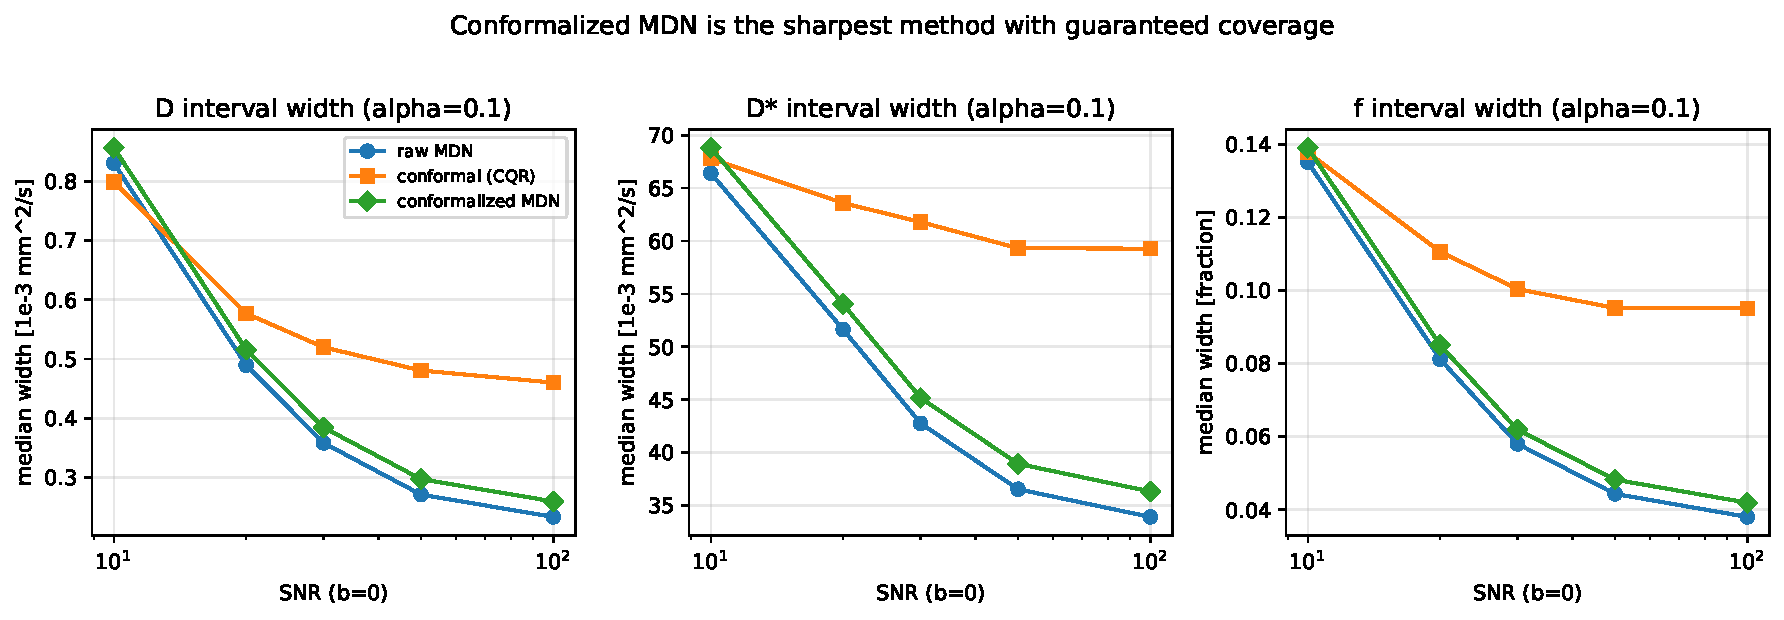
\includegraphics[width=0.78\linewidth]{figures/sharpness_vs_snr.pdf}
\caption{Median interval width vs SNR. Conformalized-MDN is the sharpest method
with a guaranteed coverage level.}
\label{fig:sharpness}
\end{figure}

\begin{figure}[h]
\centering

\includegraphics[width=0.92\linewidth]{figures/robustness_shift.pdf}
\caption{(Left) worst-parameter coverage under each exchangeability break, naive
vs.\ weighted, with monitor status. (Right) SNR-severity sweep: the monitor fires
before coverage crosses the failure line.}
\label{fig:shift}
\end{figure}

\begin{figure}[h]
\centering

\includegraphics[width=0.92\linewidth]{figures/invivo_demo.pdf}
\caption{In-vivo qualitative demo (synthetic stand-in). (Left) the conformal
$\Dstar$ band balloons with the plug-in $\hat{\Dstar}$. (Right) the heavy-tailed
$\Dstar$ band-width distribution; the deployment monitor fires on the transfer.}
\label{fig:invivo}
\end{figure}

\begin{figure}[h]
\centering
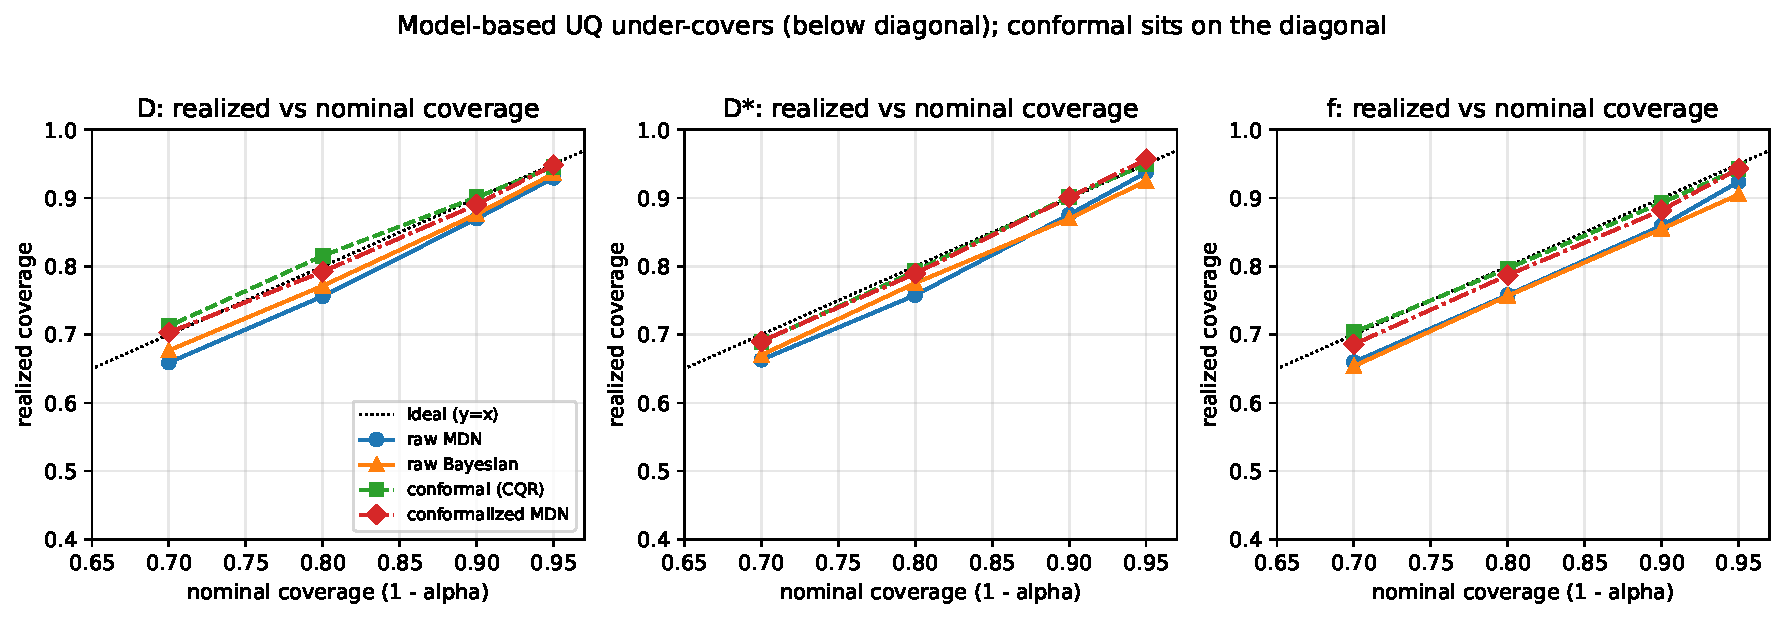
\includegraphics[width=0.78\linewidth]{figures/coverage_vs_nominal.pdf}
\caption{Realized vs nominal coverage per parameter. Raw model-based methods sit
below the diagonal (overconfident); conformal and conformalized methods sit on it.}
\label{fig:coverage}
\end{figure}

\begin{figure}[h]
\centering
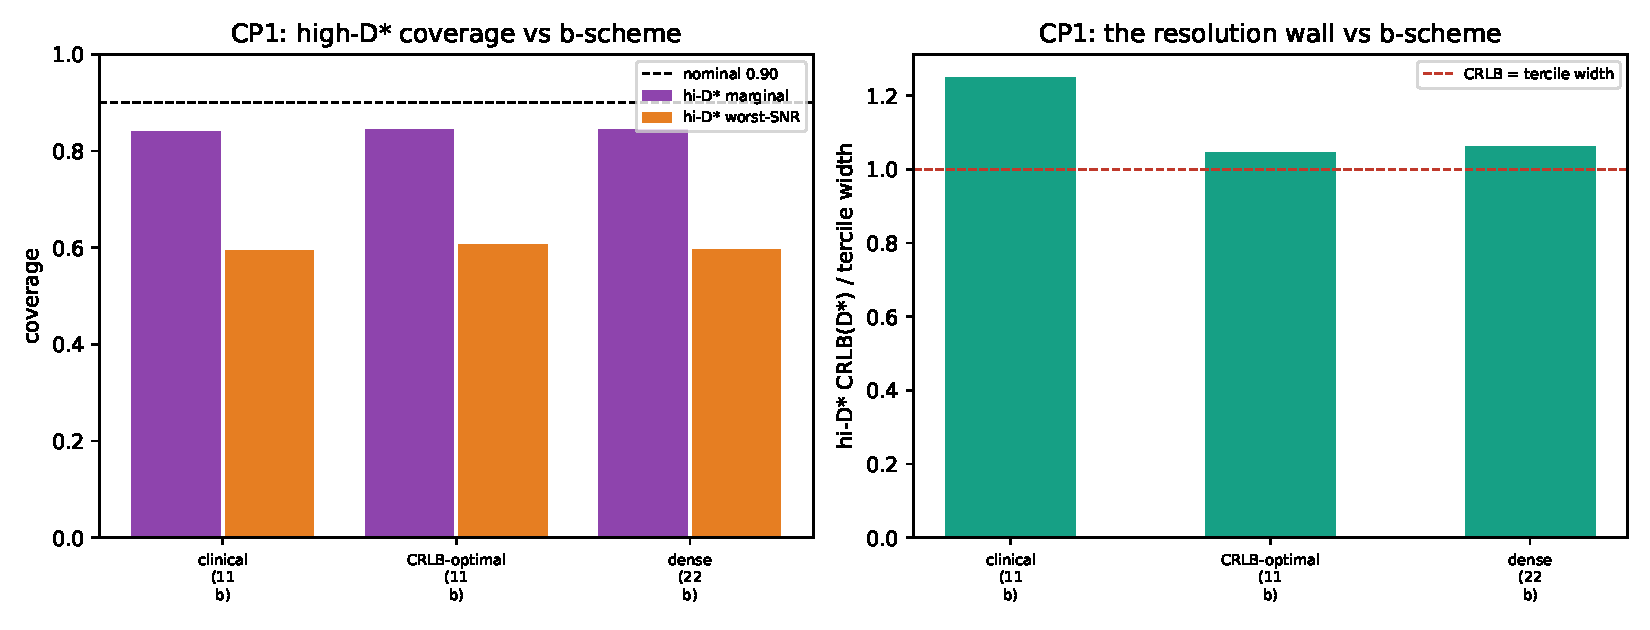
\includegraphics[width=0.92\linewidth]{figures/acquisition_wall.pdf}
\caption{(Left) high-$\Dstar$ coverage vs.\ b-scheme. (Right) the resolution ratio
CRLB($\Dstar$)/tercile-width stays at or above unity for every scheme (the
CRLB-optimal band dips to $0.97$): acquisition moves the regime to the resolution
threshold, not past it.}
\label{fig:acq}
\end{figure}

\begin{figure}[h]
\centering
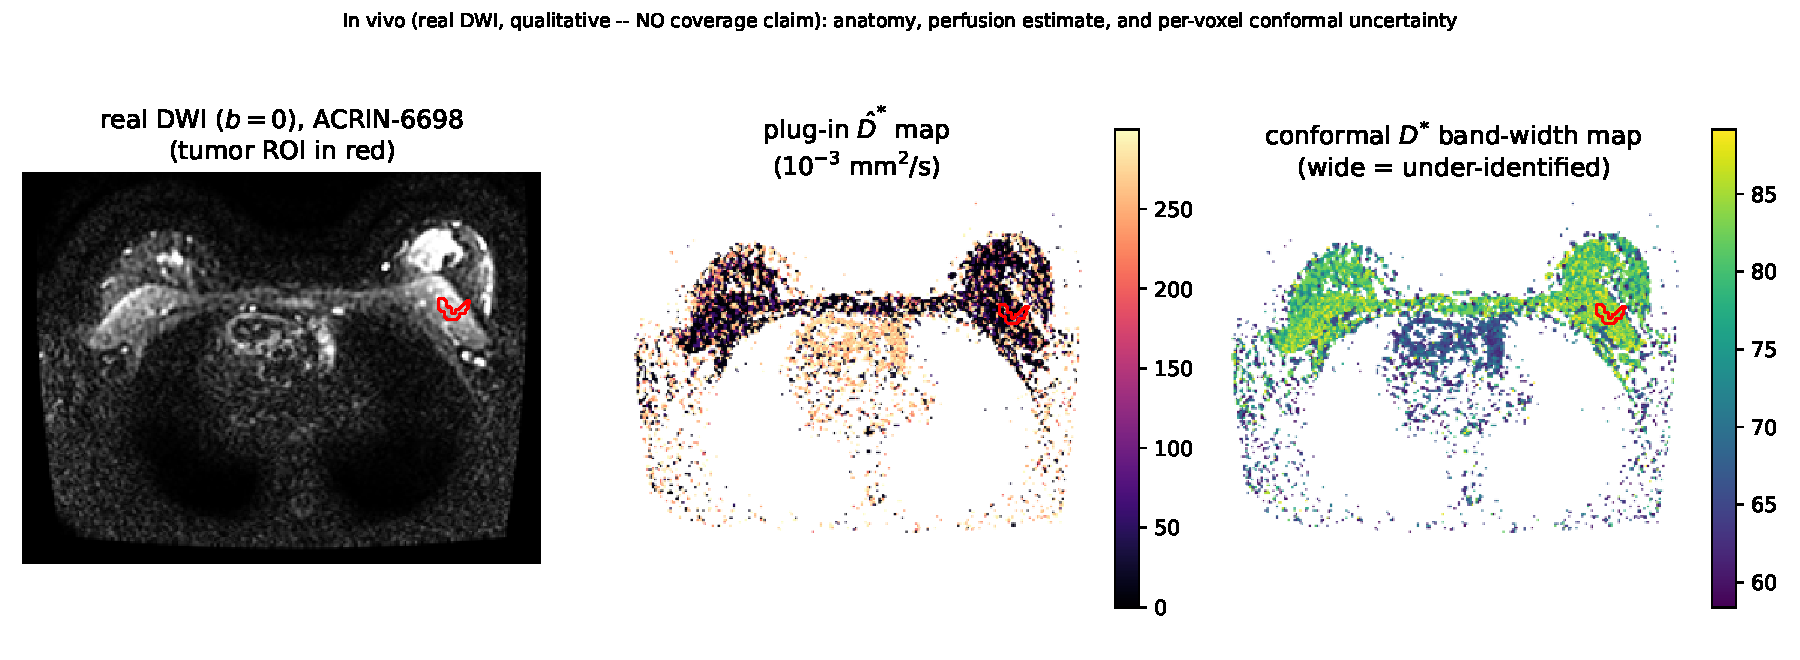
\includegraphics[width=\linewidth]{figures/invivo_real_maps.pdf}
\caption{Actual in-vivo images (ACRIN-6698 / I-SPY2 Breast DWI; one slice;
qualitative, no coverage claim). (Left) real $b{=}0$ DWI with the whole-tumor ROI in
red; (middle) the plug-in $\hat{\Dstar}$ perfusion map; (right) the per-voxel
conformal $\Dstar$ band-width map---wider where the perfusion compartment is
under-identified. The synthetic 22-value-calibrated monitor (not shown here) fires
on this data; see Fig.~\ref{fig:invivo-real}.}
\label{fig:invivo-maps}
\end{figure}

\end{document}
